\documentclass[conference]{IEEEtran}
\IEEEoverridecommandlockouts

\usepackage{cite}
\usepackage{amsmath,amssymb,amsfonts}
\usepackage{graphicx}
\usepackage{textcomp}
\usepackage{booktabs}
\usepackage{array}
\usepackage[hidelinks]{hyperref}

\newcommand{\dataset}[1]{\texttt{#1}}

\hyphenation{Urban-Sound Fast-API Air-flow Py-Spark Light-GBM Res-Net Hugging-Face}

\begin{document}

\title{An End-to-End MLOps Pipeline for Urban Sound Classification}

\author{\IEEEauthorblockN{Risan Raja}
  \IEEEauthorblockA{Indian Institute of Technology Madras\\
Chennai, India}}

\maketitle

\begin{abstract}
  This report describes a production-style machine learning operations (MLOps) system for ten-class urban sound event classification on UrbanSound8K.
  A host-side Apache Airflow DAG with LocalExecutor downloads parquet clips from Hugging Face Hub, cleans and augments waveforms, extracts tabular and log-mel features with PySpark in local mode, and trains four models under Optuna and MLflow: random forest, XGBoost, LightGBM, and a ResNet-18 convolutional network.
  The winning artifact is a ResNet-18 with holdout F1-macro \(0.876\) and official 10-fold CV F1-macro \(0.818\pm 0.040\).
  Dataset intermediates and trained weights are versioned on Hugging Face Hub.
  A FastAPI service inside Docker Compose exposes \texttt{/health}, \texttt{/metrics}, and \texttt{/predict}; Prometheus and Grafana scrape request, latency, class, confidence, and drift series, and each prediction is written as structured JSON.
  GitHub Actions lint, test, and build the API image.
  The project was completed solo under an approved exception to the course team-size rule.
\end{abstract}

\begin{IEEEkeywords}
  MLOps, audio classification, Airflow, PySpark, MLflow, FastAPI, UrbanSound8K
\end{IEEEkeywords}

\section{Problem Statement}
\label{sec:problem}

Urban environments are rich environments with mechanical, social, and emergency sounds to be classified from a short waveform by the deployed classifier.
The problem of engineering is to build upon a parquet dump a served model with an audit trail: whose training was done by whom with what hyperparameters on which fold split and how does the served model behave in live API.

The use case of classification in this project is to classify clips of UrbanSounds8K~\cite{salamon2014urbansound}.
The clip is received as a \texttt{.wav} file and returned class, confidence value, the name of the served model, end-to-end latency, and full probability vector for the all ten classes.
Under the hood of the provided API there is orchestrated data path, two types of features, comparison of four models, experiment tracking, remote versioning, model serving via containers and request-level monitoring.

The list of required components in course brief includes nine items: version control; airflow-orchestrated pipeline together with spark, kafka, or beam; data processing; comparison of at least two models using MLflow; dataset and models versioning (DVC or its alternatives); FastAPI or Flask plus Docker; logging with Prometheus, Kibana, drift detection, performance monitoring or latency/prediction logging; CI/CD; README.
Next sections describe the chosen solution for the components and explain the deviations from the typical approach to compose everything.
The Table~\ref{tab:brief} gives short version of these descriptions.

\begin{table}[!t]
  \renewcommand{\arraystretch}{1.12}
  \setlength{\tabcolsep}{2.5pt}
  \caption{Brief component versus what shipped}
  \label{tab:brief}
  \centering
  \begin{tabular}{>{\raggedright\arraybackslash}p{0.28\columnwidth}
    >{\raggedright\arraybackslash}p{0.66\columnwidth}}
    \toprule
    Brief item & This repo \\
    \midrule
    Git + Hub & Feature branches, semantic commits, GitHub remote \\
    Airflow + DE tool & Host LocalExecutor DAG; PySpark local UDFs \\
    Processing & Decode, resample, peak-norm; train-fold augment \\
    \(\geq\)2 models + MLflow & RF, XGBoost, LightGBM, ResNet-18; SQLite tracker \\
    Versioning & HF dataset prefixes + model repo (DVC documented) \\
    Serve + Docker & FastAPI three-route API in Compose \\
    Monitoring & Prometheus, Grafana, JSON logs, KS/PSI drift \\
    CI/CD & GitHub Actions: ruff, pytest, image build/push \\
    README & Setup script + multi-OS install; architecture, API, Docker, tree \\
    \bottomrule
  \end{tabular}
\end{table}

\section{Dataset}
\label{sec:dataset}
\label{ds:urbansound}
The UrbanSound8K dataset consists of \(8{,}732\) labeled audio clips, each no more than four seconds in length, taken from the \dataset{freesound} archive and annotated with ten different labels: \dataset{air conditioner}, \dataset{car horn}, \dataset{children playing}, \dataset{dog bark}, \dataset{drilling}, \dataset{engine idling}, \dataset{gun shot}, \dataset{jackhammer}, \dataset{siren}, and \dataset{street music}~\cite{salamon2014urbansound}.
For each clip, there is an attribute called \dataset{fold} which takes an integer value in \(\{1,\ldots,10\}\).
The dataset follows an official cross-validation setting where no two clips from the same recording file are placed into the same split, contrary to a purely randomized splitting approach.

The pipeline does not pull the original data as a git submodule. Instead it loads the parquet representation of the above-mentioned clips from the Hub dataset \dataset{risan-raja-iitm/urbansound8k} which is simply a mirror of \dataset{danavery/urbansound8k} dataset, licensed under CC-BY-NC-4.0.

Audio data is stored in Hugging Face \texttt{Audio} structs in sixteen parquet files~\cite{huggingface}.
The validated columns include \texttt{audio} (in bytes and path), \texttt{slice\_file\_name}, \texttt{fsID}, \texttt{start}, \texttt{end}, \texttt{salience}, \texttt{fold}, \texttt{classID}, and \texttt{class}.
The manifest file \texttt{.manifest.json} is downloaded by a SHA-based downloader, which also verifies the row count (\(8{,}732\)), fold range, and number of classes before any subsequent pipeline step executes.
A git submodule of the raw archives would have entailed cloning multi-gigabytes worth of files and installing \texttt{git-lfs} on every grader machine and CI runner; using Hub ensures a lightweight git repository and requires no Kaggle authentication.

Raw parquet files are regarded as an upstream cache, not as a versioned dataset for this project.
What this project versions on Hugging Face Hub are interim waveforms, processed features, and model artifacts produced by \emph{this} pipeline.
Class imbalance is present (the fewest classes being gun shot and car horn) – this is the reason behind training-fold augmentation and the reason for using macro-F1 instead of accuracy.

\section{System Architecture}
\label{sec:arch}

Figure~\ref{fig:arch} is the runtime map: data preparation and training on the host, serving and monitoring in Docker Compose.
Airflow and PySpark run on the host virtualenv.
Docker Compose runs only the API, MLflow UI, Prometheus, and Grafana.
The brief requires Airflow, not Airflow-in-Docker.

LocalExecutor runs callables of the DAGs in the same Python instance as the training of ResNet-18, hence Apple Silicon MPS can be used and there is no secondary, CPU-only torch build in a Linux container~\cite{airflow}.
Celery, Redis, and Flower would introduce failure modes where there is no second worker machine.

PySpark is the second tool for data engineering~\cite{zaharia2010spark,zaharia2016spark}.
PySpark is launched as \texttt{master=local[*]} (actually \texttt{local[2]} in \texttt{config/config.yaml}) within a \texttt{PythonOperator}, not as a separate cluster.
There are eight thousand short videos and there is no need for Spark cluster; the UDF interface will remain the same even if one is pointed at later.

MLflow makes use of the \texttt{./mlflow/} SQLite backend store, bind-mounted to the Compose service so that host training and the container-based MLflow UI can access one common file~\cite{zaharia2018mlflow}.
The SQLite backend store is a single-writer store, i.e., it should not be accessed by both host training and the containerized \texttt{mlflow server} simultaneously.
Accordingly, the DAG sets \texttt{MLFLOW\_TRACKING\_URI=http://localhost:5001} once the Compose tracker is running.

The versioning strategy is based on two Hub repositories.
The existing dataset repository holding the raw parquet files gets \texttt{interim/} and \texttt{processed/} prefixes appended to it in the future.
The other repository of the \texttt{model} type, which is \texttt{risan-raja-iitm/urbansound8k-models}, holds four trained directories as well as \texttt{winner.json} and \texttt{winner/}.
``DVC or equivalent'' is allowed in the guidelines, so Hub dataset and model repositories are the primary equivalent.

\begin{figure*}[!t]
  \centering
  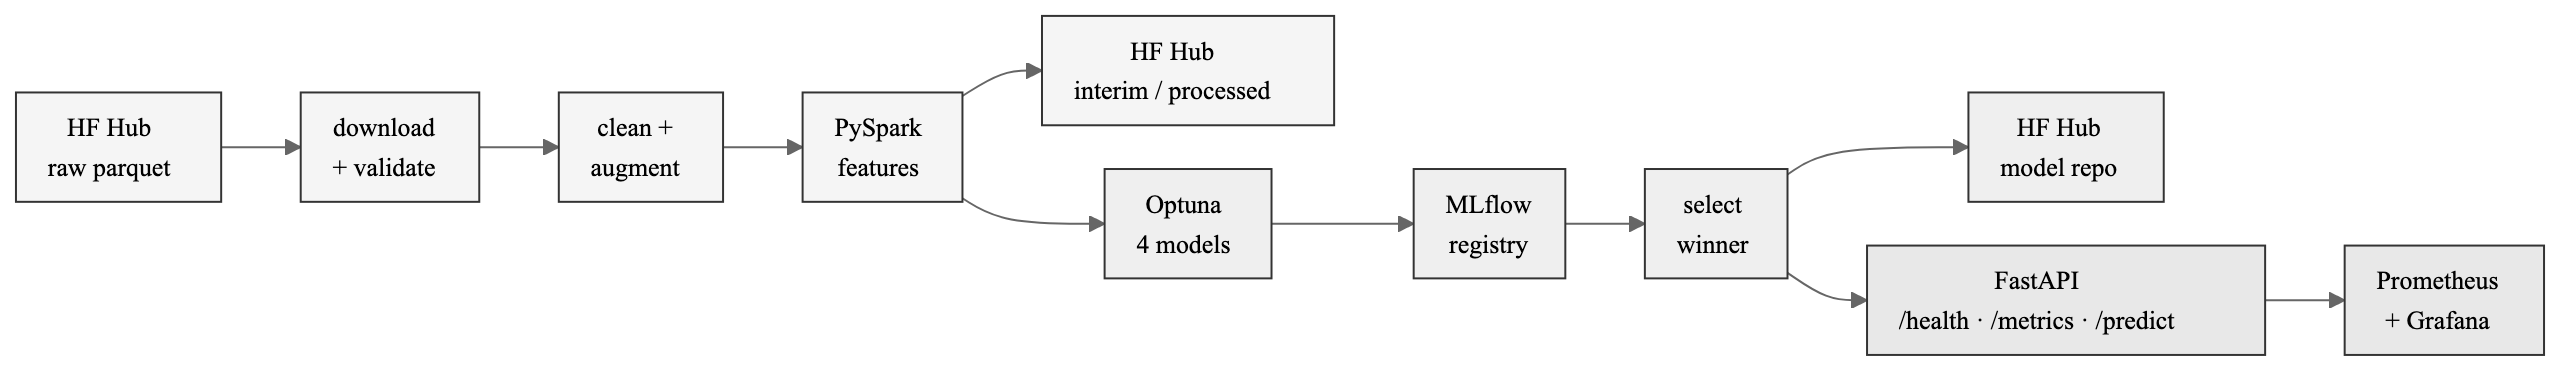
\includegraphics[width=\textwidth]{figures/architecture.png}
  \caption{System architecture. Hugging Face Hub stores raw and processed data plus model artifacts; Airflow/LocalExecutor and PySpark run on the host; FastAPI, Prometheus, and Grafana run in Compose.}
  \label{fig:arch}
\end{figure*}

\section{Data Pipeline}
\label{sec:pipeline}

The DAG \texttt{audio\_classification} is manual (\texttt{schedule=None}).
Figure~\ref{fig:dag} shows the task graph: a linear ingest/feature spine, a four-way fan-out for training, then fan-in for winner selection and Hub pushes.
Each callable changes into the repository root and imports the corresponding \texttt{src} module only inside the task body, so the scheduler can parse the DAG without loading torch or Spark.
\texttt{preprocessing.enabled} and \texttt{spark.enabled} in \texttt{config.yaml} can turn the heavy stages into no-ops so a demo rerun reuses \texttt{data/interim} and \texttt{data/processed} instead of spending an hour re-deriving wavs.

\begin{figure*}[!t]
  \centering
  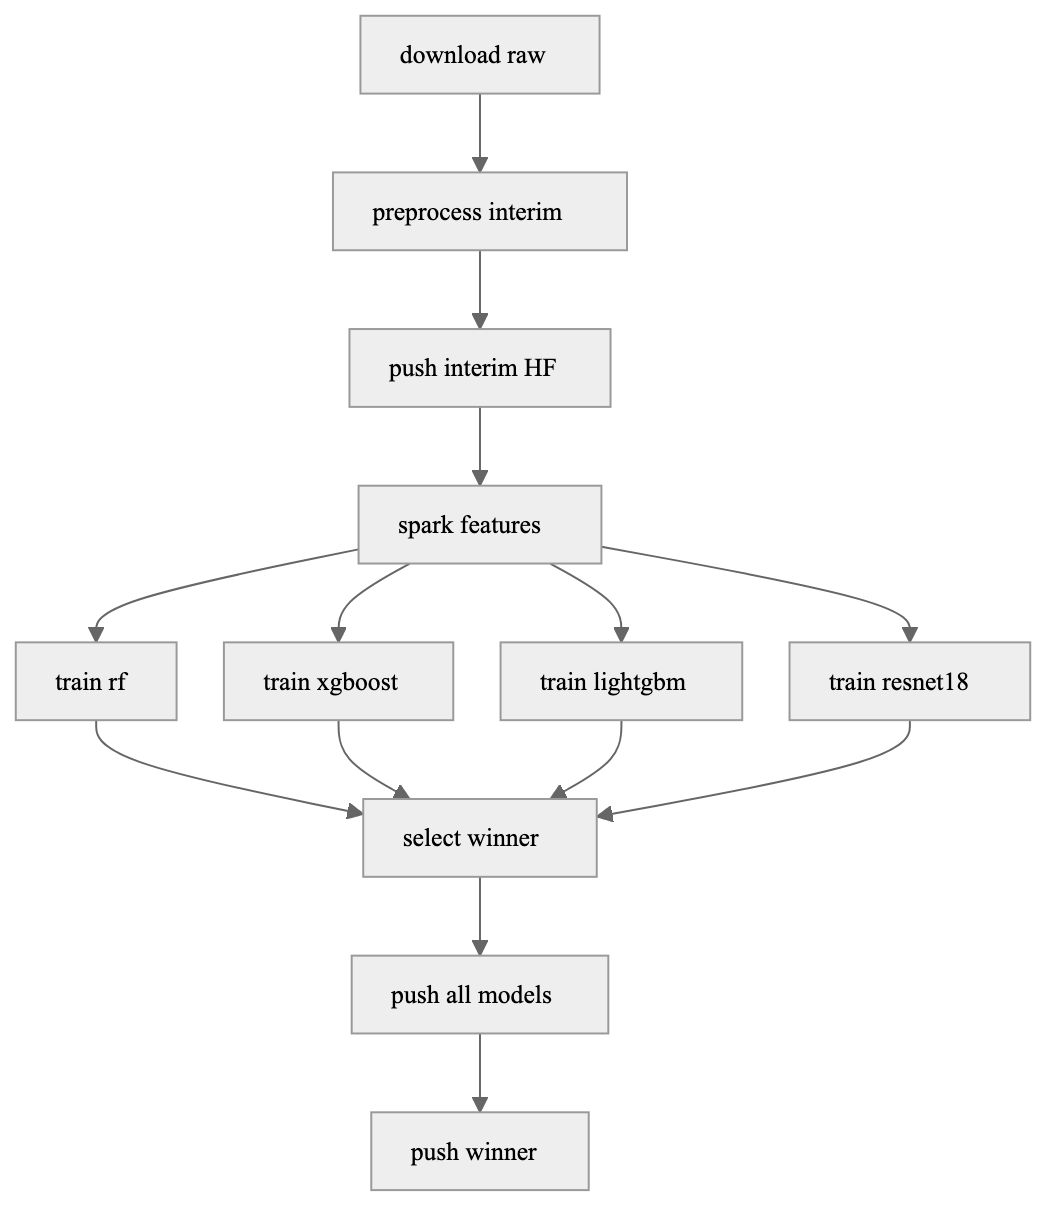
\includegraphics[width=0.72\textwidth]{figures/dag.png}
  \caption{Airflow DAG \texttt{audio\_classification}. Sequential ingest through Spark feature extraction, fan-out to four parallel \texttt{train\_*} tasks, fan-in at \texttt{select\_winner}, then Hub pushes.}
  \label{fig:dag}
\end{figure*}

\subsection{Cleaning and augmentation}

The raw clips come in with different sample rates, one or two channels, and some with either missing or all-zero payloads.
The preprocessor unpacks the bytes using \texttt{soundfile}, filters out empty vectors, converts stereo to mono via mean, resamples to \(16\,\mathrm{kHz}\) using librosa~\cite{mcfee2015librosa}, and peak-normalizes.
Clips without any content (amplitude zero) throw exceptions; they do not get imputed.
Corrupted or empty audio throws loudly instead of turning into a vector of zeros later on to resemble a class label.

Fold 10 is held out during preprocessing and never gets augmented.
Each training fold is copied once more with augmentations performed with an \texttt{audiomentations} compose consisting of Gaussian noise, pitch shift of \(\pm 2\) semitones, and time stretch in \([0.9, 1.1]\) with probabilities of \(0.5\) for each operation.
Seeds are generated by hashing a base seed, clip key, and a copy index so that experiments are reproducible.
These augmented wavs along with a \texttt{metadata.parquet} (containing the \texttt{is\_augmented} flag) compose \texttt{data/interim}.

\subsection{PySpark feature extraction}
The extractor starts a local SparkSession and maps each absolute wav path through a Python UDF~\cite{zaharia2016spark}.
Every clip is padded or truncated to \(4\,\mathrm{s}\).
Two feature families are written:

\textbf{Tabular.} Thirteen MFCCs and their first-order deltas, twelve chroma bins, spectral centroid, bandwidth, rolloff, and zero-crossing rate, each reduced to mean and standard deviation (\(84\) scalars).
These feed the tree models~\cite{pedregosa2011sklearn}.

\textbf{Log-mel.} A \(128\times 126\) log-mel spectrogram (\(n_{\mathrm{fft}}=1024\), hop \(512\)) for the CNN, with per-dataset mean/variance stored for serving-time normalization.

The same librosa helpers live in \texttt{src/data\_pipeline/audio\_features.py} so the API can rebuild features from an uploaded wav without importing PySpark.

\subsection{Fold protocol at train time}
Training reads processed parquet and applies the configured holdout:
folds \(1\)--\(8\) for fitting, fold \(9\) for Optuna validation, fold \(10\) for the reported eval metrics.
When \texttt{training.cv.enabled} is true, the selected hyperparameters are re-evaluated under official 10-fold CV (train on nine folds, test on the held-out fold, rotate).
Winner selection prefers \texttt{cv\_f1\_macro\_mean} when present, otherwise holdout F1-macro.

\section{Model Development}
\label{sec:models}

Four models are trained, which is more than the brief's minimum of two, and they sit on two representations rather than two hyperparameter grids of the same learner.
Figure~\ref{fig:lifecycle} is the per-model lifecycle shared by the tabular baselines and ResNet-18.

\begin{figure*}[!t]
  \centering
  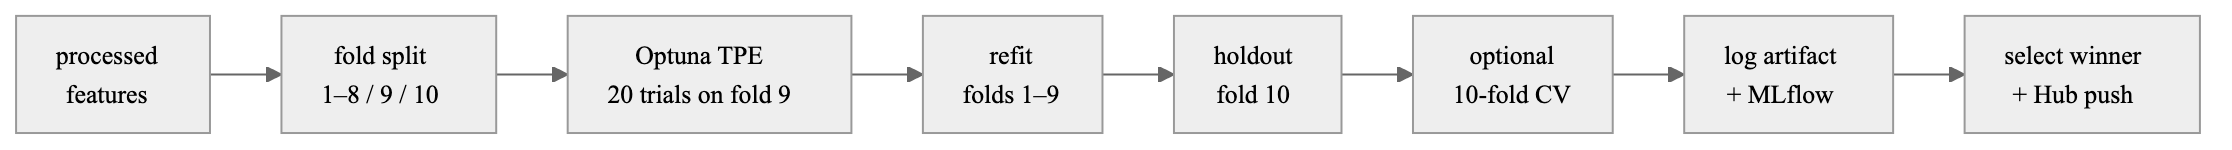
\includegraphics[width=\textwidth]{figures/lifecycle.png}
  \caption{Per-model development lifecycle. Optuna maximizes fold-9 macro-F1 over 20 trials; best hyperparameters refit folds 1--9, score fold 10, optionally run 10-fold CV, then log to MLflow and enter winner selection.}
  \label{fig:lifecycle}
\end{figure*}

Random forest~\cite{breiman2001rf}, XGBoost~\cite{chen2016xgboost}, and LightGBM~\cite{ke2017lightgbm} process the \(84\)-dimensional table vector after being fitted via \texttt{StandardScaler} on the training folds only.
Class weight vectors calculated from Optuna training folds balance the minority class gun-shot and car-horn data points while training the trees.
ResNet-18~\cite{he2016resnet} processes the normalized log-mel in form of a single-channel image; residual weights pre-trained on ImageNet are fine-tuned for ten classes with patience \(5\).

The search spaces reside in the training modules rather than \texttt{config.yaml} file, so the configuration file remains a list of paths and fold integers.
Optuna performs \(20\) trials for each model~\cite{akiba2019optuna}.
Random forest searches \(n_{\mathrm{estimators}}\in\{100,\ldots,400\}\), max tree depth \(4\)--\(24\), leaf nodes number, and \texttt{max\_features}.
XGBoost and LightGBM search max tree depth, log-transformed learning rate, row/column subsampling, and \(L_2\) regularization; both are histogram-based algorithms and hence do not require a GPU, allowing parallel execution of four Airflow tasks.
The CNN search space is purposefully smaller: log-uniform learning rate in \([10^{-5}, 3\times 10^{-4}]\) and batch size \(\{16,32\}\).
A twenty-trial search over residual architecture would have blown the wall clock.

After the best trial, the code refits on folds \(1\)--\(9\) (train plus the Optuna val fold) and scores fold \(10\).
That refit is what \texttt{models/<name>/} and the MLflow registry actually store.
Nested MLflow runs keep each Optuna trial visible under the parent study  and see why LightGBM beat random forest without opening four notebook dumps.

Table~\ref{tab:search} lists the searched knobs.
The spaces are wide enough that twenty trials sample rather than exhaust the grid.

\begin{table}[!t]
  \renewcommand{\arraystretch}{1.12}
  \setlength{\tabcolsep}{2.5pt}
  \caption{Optuna search spaces (20 trials each)}
  \label{tab:search}
  \centering
  \begin{tabular}{ll}
    \toprule
    Model & Tuned knobs \\
    \midrule
    RF & trees \(100\)--\(400\); depth \(4\)--\(24\); leaf; \texttt{max\_features} \\
    XGBoost & trees; depth \(3\)--\(12\); \(\eta\); subsample; \(\lambda\) \\
    LightGBM & trees; depth; \(\eta\); leaves \(16\)--\(128\); min child \\
    ResNet-18 & \(\eta\in[10^{-5},3\times10^{-4}]\); batch \(\{16,32\}\) \\
    \bottomrule
  \end{tabular}
\end{table}

Each training run records its hyperparameters and the fold-based performance measures called for by the assignment: accuracy, macro precision, macro recall, macro F1, weighted F1, one-vs-rest ROC-AUC, and a confusion-matrix image (.png).
The model object or scaler/mel stats or label map mapping, respectively, is saved into \texttt{models/<name>/} and registered in MLflow.
Once all four \texttt{train\_*} jobs have completed, \texttt{select\_winner} moves the winning folder to \texttt{models/winner/}, saves \texttt{winner.json} (the winning model name, the evaluation scores, the MLflow \texttt{run\_id} and dataset \texttt{SHA}), and marks the production alias in MLflow Registry.

OpenMP/BLAS thread limits are loaded from the \texttt{.env} file in \texttt{src/models/runtime\_env.py} prior to importing sklearn, XGBoost, LightGBM, and torch.
Otherwise, four parallel train tasks from Airflow will overload the host.

\section{Deployment}
\label{sec:deploy}
This API Service uses three endpoints available via FastAPI~\cite{fastapi}. It is containerized using the \texttt{docker/Dockerfile.api} (\texttt{python:3.11-slim}) Docker image and published on host port \(8000\).

\texttt{/health} gives back \texttt{\{``status'': ``ok''\}}, even if the weights are not loaded, which allows an orchestrator to separate ``process up'' and ``model ready'' cases.
\texttt{/metrics} gives out metrics in Prometheus text format.
\texttt{/predict} takes a multipart \texttt{.wav}.
Files greater than \(8\,\mathrm{MiB}\), empty files and files which are not \texttt{.wav} in the extension nor \texttt{audio/wav} (and some very close variants) in MIME type will result in a HTTP error code of \(400\) or \(413\).
No winner will cause a HTTP status of \(503\).
When successful, the body will contain the Pydantic model: \texttt{label}, \texttt{confidence}, \texttt{model\_name}, \texttt{latency\_ms}, and \texttt{probabilities}.

Startup resolves artifacts in order: \texttt{models/winner/}, then \texttt{models/<name>/} from \texttt{winner.json}, then a Hub snapshot of the model repo into a cache directory.
A CNN directory must contain \texttt{model.pt}, \texttt{mel\_stats.json}, and \texttt{label\_map.json}; a tabular directory must contain \texttt{model.joblib}, \texttt{scaler.joblib}, and \texttt{label\_map.json}.

CNN and tabular families share \texttt{predict\_clip}: decode, resample, pad or truncate, then either a torch forward pass or a scaler-plus-tree \texttt{predict\_proba}.
Compose bind-mounts \texttt{config/} and \texttt{models/} read-only and loads \texttt{.env}.
\texttt{DA5402W\_CONFIG} and \texttt{DA5402W\_MODELS\_DIR} override those mounts when the same code is run under uvicorn on the host.
A helper, \texttt{make demo-predict}, posts three UrbanSound8K clips per class so Grafana is not an empty shell during a demo.

\section{Monitoring}
\label{sec:monitor}

Of the four that has been implemented here - Prometheus scrape metrics, API latency histograms, per-prediction JSON logs, and a KS/PSI drift detector - Grafana is configured at the top layer (not a requirement of this brief) and therefore you will be able to demonstrate via a viva request rate, error ratio, p50/p95/p99 latency, predicted-class mix, mean confidence, class-mix PSI, confidence KS, and process CPU/memory without having to click-through PromQL.

Refer to counters/histograms \texttt{predict\_requests\_total}, \texttt{predict\_errors\_total}, \texttt{predict\_class\_total\{class\_name\}}, \texttt{predict\_latency\_seconds}, \texttt{predict\_confidence}~\cite{rabenstein2015prometheus}.
Similarly, check the drift gauges \texttt{drift\_psi\_class}, \texttt{drift\_ks\_confidence}, and \texttt{drift\_window\_size}.

API Overview is loaded from \texttt{docker/grafana/provisioning/} on each boot of the container. Each request (both success/failure) is recorded into stdout as one json object containing timestamp, status, label, confidence, model name, latency, and filename.

Rolling live drift uses a window of \(100\) successful predictions compared to \texttt{models/drift\_reference.json}.
Class-mix PSI is calculated using the official fold-10 label prior (UrbanSound8K counts when \texttt{data/processed} is absent). Confidence KS uses fold-10 quantile samples where these exist in the reference; otherwise it is set to none.
CNN serving path does not extract the \(84\)-dimensional tabular vector so, although we do have an online CLI (\texttt{python -m src.monitoring.drift\_cli}), which calculates both PSI and K-S against processed parquet files, the former is an offline cost.

\section{CI/CD}
\label{sec:cicd}

\texttt{.github/workflows/ci.yml} runs on pull requests and pushes to \texttt{main}.
Three jobs chain: \texttt{ruff check}, \texttt{pytest -m ``not integration''}, then a Docker build of \texttt{Dockerfile.api}.
On \texttt{main} the image is pushed to GitHub Container Registry as \texttt{ghcr.io/risan-raja-iitm/da5402w-api} with \texttt{latest} and git-SHA tags.
PR builds verify the Dockerfile without publishing.

Integration tests that hit the Hub or a live Spark session are marked and excluded so CI stays deterministic on a GitHub-hosted runner.
The workflow does not boot the full Compose stack.
A multi-service Airflow-plus-API boot inside that runner is a flaky source that does not improve the Dockerfile check the brief actually needs.

\section{Reproducibility}
\label{sec:repro}
The intention behind the design of the git tree is to clone without the seven gigabytes of wav files.
In order to obtain the graded bootstrap path, the steps are as follows:
Clone, followed by \texttt{make setup} (or \texttt{bash scripts/setup.sh}) : the script first verifies whether python version 3.13+ , uv, and java version 17 exist on your computer; then, when necessary, it creates .env from .env.example; finally, it executes uv sync --locked --group dev.
On linux and macos one should run it native; on windows, one needs to install WSL2 (the preferred option) or Git Bash in order to execute the script.
For Torch running under linux/windows, it will run exclusively as a cpu-version by virtue of the uv indexes in pyproject.toml.
For Torch running under macos, one can train models hosted on the machine with mps.
As stated above, the only additional package that pyspark requires is java version 17.
\texttt{make compose} starts the api, mlflow on host port 5001 (port 5000 is occupied by airplay on macos), prometheus, and grafana.
\texttt{make airflow} initiates LocalExecutor with metadata stored within git-ignored directory .airflow/.
\texttt{make pull-winner} snapshots both winner.json and winner/ from the model repository if either of these directories does not currently exist.

If a user wishes to solely get the score for a clip he/she will never need to start spark.
The serving container rebuilds the features from the inputted bytes that were loaded onto the api using shared librosa helper functions. The scaler or mel-statistics that traveled with the winner are used during this process. This is why feature code was moved outside of the spark module: If we imported \texttt{pyspark} inside of our very slim api image, then we would have also pulled java into a service that only requires numpy and librosa.

All configuration is contained in one yaml file.
Lists of folds, trial counts, spark heap size, hub repository ids, and push flags are included.
Secrets remain in \texttt{.env} (huggingface token, grafana admin pass).
If huggingface token and grafana admin password variables are unset in the env file, grafana defaults to \texttt{admin/admin}.

\section{Results and Discussion}
\label{sec:results}

Table~\ref{tab:results} reports fold-\(10\) holdout metrics after Optuna and the subsequent official 10-fold CV mean and standard deviation of macro-F1.
Numbers are taken from \texttt{models/*/metrics.json}.

\begin{table}[!t]
  \renewcommand{\arraystretch}{1.15}
  \setlength{\tabcolsep}{3pt}
  \caption{Holdout (fold 10) and 10-fold CV. Winner selected by CV F1-macro.}
  \label{tab:results}
  \centering
  \begin{tabular}{lcccc}
    \toprule
    Model & Acc. & F1-mac. & AUC & CV F1 \\
    \midrule
    RF & 0.720 & 0.721 & 0.956 & \(0.655\pm 0.043\) \\
    XGBoost & 0.771 & 0.776 & 0.961 & \(0.689\pm 0.053\) \\
    LightGBM & 0.780 & 0.788 & 0.960 & \(0.697\pm 0.054\) \\
    ResNet-18 & \textbf{0.864} & \textbf{0.876} & \textbf{0.991} & \(\mathbf{0.818\pm 0.040}\) \\
    \bottomrule
  \end{tabular}
\end{table}

ResNet-18 was also found to be the top model based on both the hold-out F1-macro score (\(0.876\)) as well as the CV F1-macro score (\(0.818 \pm 0.040\)).
LightGBM had the highest F1 scores among all the table-based models, at hold-out F1 (\(0.788\)) and CV F1 (\(0.697 \pm 0.054\)). XGBoost was nearly tied with LightGBM at CV (\(0.689 \pm 0.053\)).
Random Forest performed usefully as a baseline at both hold-out F1 (\(0.721\)) and CV F1 (\(0.655 \pm 0.043\)), however it did so significantly behind both of the two boosting algorithms.

This is why we have CV in our DAG; this is why the gap between the evaluation metrics of each of these methods exists.
We happen to have used Fold 10 as an example of how good the evaluation metric could be; if you were to rotate the test set, we find that the macro-F1 of ResNet-18 decreases by approximately \(0.06\), while the macro-F1 of each of the tabular models decreases by approximately \(0.09\). The standard deviation across folds for ResNet-18's CV is \(0.04\).
Therefore, using only results from one fold would potentially overestimate the quality of what will actually be deployed.
Using only results from CV would hide where the Optuna objective function was optimized (on fold 9), as well as the published hold-out result (from fold 10), but a user could still compute either of those values again from \texttt{winner.json}.

Figure~\ref{fig:cm-cnn} shows ResNet-18’s confusion matrix for the hold-out set.
All of the lightness in the upper right triangle comes from car horn and gunshot – they are minority classes, and thus will appear less intense on a simple count-per-class heatmap even when their true recall is adequate.
The mistakes shown are mostly those that UrbanSound8K papers typically show: leakage of sirens into both children playing and dog barking; exchange of mass between drilling and jackhammer; leakage of engine idling into air conditioner; leakage of street music into children playing.
These mistakes occur because these classes overlap in terms of frequency band, as well as due to background noise within the original audio files.

\begin{figure}[!t]
  \centering
  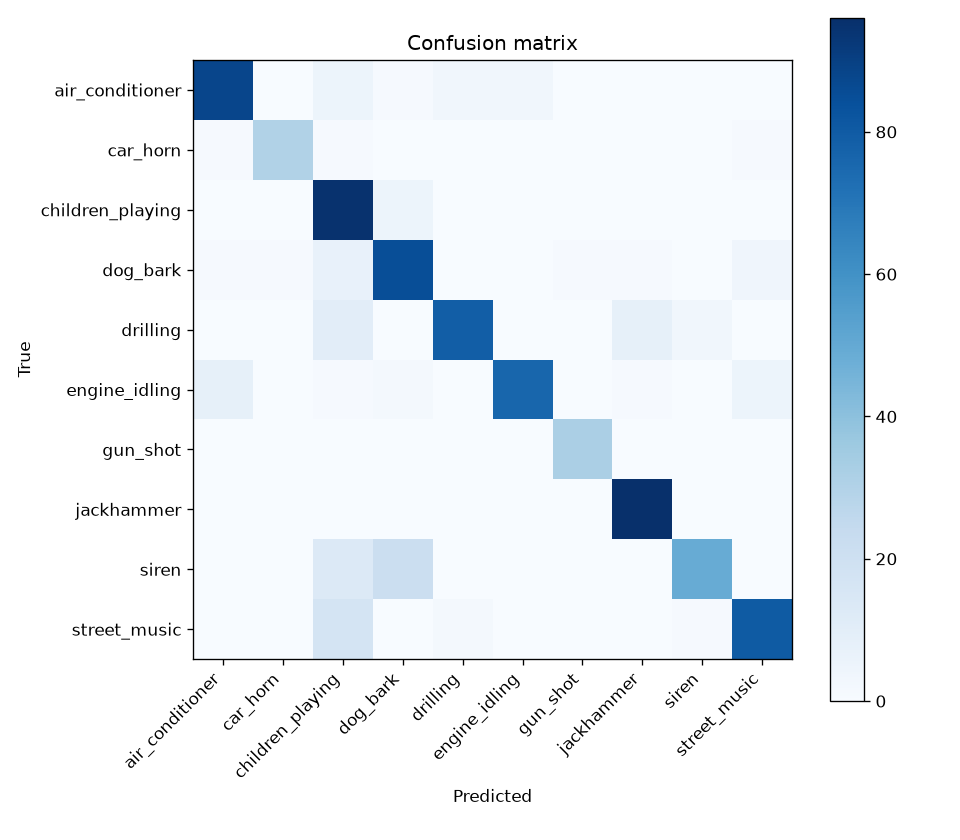
\includegraphics[width=\columnwidth]{figures/cm_resnet18.png}
  \caption{ResNet-18 holdout confusion matrix (fold 10). Mechanical pairs (drill/jackhammer, engine/AC) and siren versus vocal street scenes remain the main errors.}
  \label{fig:cm-cnn}
\end{figure}

\begin{figure}[!t]
  \centering
  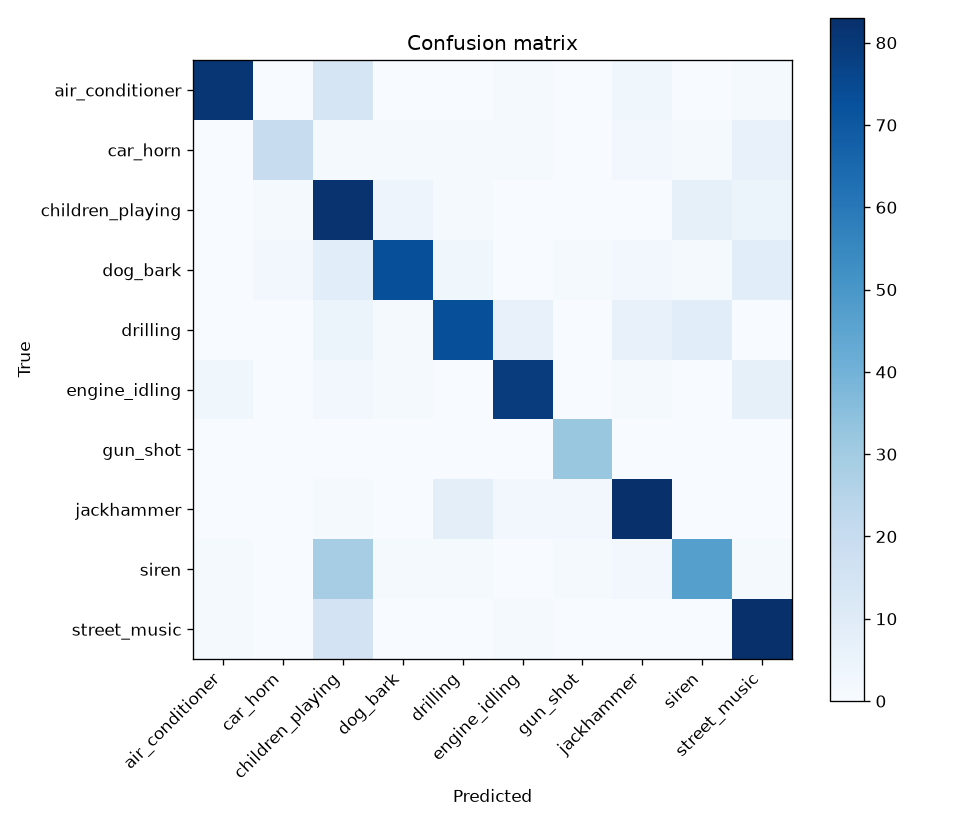
\includegraphics[width=\columnwidth]{figures/cm_lightgbm.png}
  \caption{LightGBM holdout confusion matrix. The same class pairs confuse the tabular model, with more siren\(\rightarrow\)children\_playing mass than ResNet-18.}
  \label{fig:cm-lgb}
\end{figure}

Figure~\ref{fig:cm-lgb} is LightGBM on the same fold.
The error structure is the same family, with a thicker siren-to-children-playing off-diagonal.
The CNN's extra \(0.09\) holdout F1 comes from cutting the confusions that a bag of MFCC and chroma summaries cannot separate.

Lineage in \texttt{winner.json} records the Hub dataset id, processed-set timestamp, tabular SHA, and MLflow run \texttt{9cf8d81bed6b4ea99d91240e1e17133e}.
A later retrain that does not match that SHA is a different artifact, even if the class name is still \texttt{resnet18}.

Reproducibility for a grader is a short list: clone, \texttt{make setup}, \texttt{make pull-winner} or a local \texttt{models/winner}, \texttt{make compose}, and \texttt{curl} a sample wav.
Full training is optional; the Hub model repo is the artifact store the brief asked for.
The DAG remains the path that created those artifacts, and that is what the viva should walk.

\section{Challenges}
\label{sec:challenges}

The ``default'' airflow production sketch for putting Airflow in compose looks like the default ``production'' sketch for the development machine. A Linux API image cannot see the MPS whereas a celery worker inside of docker would be able to train resnet on cpu and make a twenty trial CNN search very expensive. Using Host LocalExecutor, along with a very thin compose file (api, tracker, scrape stack), resolved the bottlenecks and allowed the pipeline to run efficiently on local hardware.

PySpark running on the host required java 17, as well as a small driver heap (1g, 512m result cap, two partitions, batch size 512). The first realisation about PySpark - making the spark driver huge wasted ram but did not increase throughput on \(4\,\mathrm{s}\) wavs. The partitioning will provide parallelism due to having multiple partitions, not because of a \(16\,\mathrm{g}\) heap.

One of the early problems we encountered during development was that, when you have MLflow pointing to a UI at \url{http://localhost:5000} and also have the compose server running, they lock each other out. Now there is no debate about whether one would want to use \texttt{mlflow ui} to monitor the training of models while they are being trained by the workers, or if one needs to shut down compose before you write the results back to \texttt{sqlite:///mlflow/mlflow.db}. It is simply mechanical.

Four Optuna trials run in parallel and collided on OpenMP.
Setting \path{OMP_NUM_THREADS} (and related knobs) in \path{.env} and importing them before the ML stack made the difference between a clean DAG run and a stall that looked like a Spark hang.
What this project versions are interim audio, processed parquet, and the four model directories, which are the artifacts one needs to reproduce the winner without re-deriving features from scratch.

\section{Future Improvements}
\label{sec:future}

In addition to Grafana serving as a working monitoring tool, it should grow alerting rules for metrics such as error rate, p95 latency, and psi.

Composing CI can include a compose smoke test that calls /health and /predict with the same check-in wavfile as part of its smoke tests. We currently gate this smoke test to only run after a pull request has been approved.
% Currently dvc is only used as a second remote (in addition to gitlab.com); we have written documentation for how to wire up dvc.yaml stages that mirror the pipeline DAG. This would allow us to say that the workflow above can be reproduced via "equivalent means."

With respect to the model side, class-balance sampling or a siren specific augmentation could help address the off diagonal term shared between both figures.

\section*{Acknowledgment}
This submission is solo work undertaken by the author.

\bibliographystyle{IEEEtran}
\bibliography{references}

\clearpage
\onecolumn
\appendices
\section{Supplementary System Screenshots}
\label{app:screenshots}

The figures at the end of this appendix are UI captures from a completed end-to-end run.
They complement the architecture, DAG, and lifecycle diagrams in the main text by showing what a grader or operator sees in Airflow, MLflow, Hugging Face Hub, and Grafana without rerunning the full pipeline.

\subsection{Orchestration}
Figure~\ref{fig:app-airflow} shows the Airflow grid after a successful \texttt{audio\_classification} DAG run.
The graph is linear from ingest through Spark feature extraction, fans out to four parallel training tasks, then converges at winner selection and Hub push tasks.
A fully green run confirms that LocalExecutor on the host executed the fan-out without a separate worker pool.

\subsection{Experiment Tracking}
Figure~\ref{fig:app-mlflow} is the MLflow experiment view comparing all four model runs under one study.
Each run records Optuna trial metadata, fold-10 holdout metrics, optional 10-fold CV scores, confusion-matrix artifacts, and the saved model binary.
Figure~\ref{fig:app-registry} shows the Model Registry after \texttt{select\_winner}: the winning ResNet-18 carries the \texttt{Production} alias, and the registry entry matches the MLflow \texttt{run\_id} written to \texttt{winner.json}.

\subsection{Artifact Versioning on Hugging Face Hub}
Figures~\ref{fig:app-hf-dataset} and~\ref{fig:app-hf-model} document the two Hub repositories used as the primary ``DVC or equivalent'' mechanism.
The dataset repo holds pipeline outputs under \texttt{interim/} and \texttt{processed/} prefixes while raw parquet remains upstream.
The model repo stores four trained directories plus \texttt{winner.json} and \texttt{winner/}, which is what \texttt{make pull-winner} snapshots when local artifacts are absent.

\subsection{Production Monitoring}
Figure~\ref{fig:app-grafana} is the provisioned Grafana ``API Overview'' dashboard fed by Prometheus scrapes of \texttt{/metrics} and structured prediction logs.
After \texttt{make demo-predict}, panels show request rate, error ratio, latency percentiles, predicted-class mix, mean confidence, and drift gauges (\texttt{drift\_psi\_class}, \texttt{drift\_ks\_confidence}).

\clearpage
\begin{figure}[!t]
  \centering
  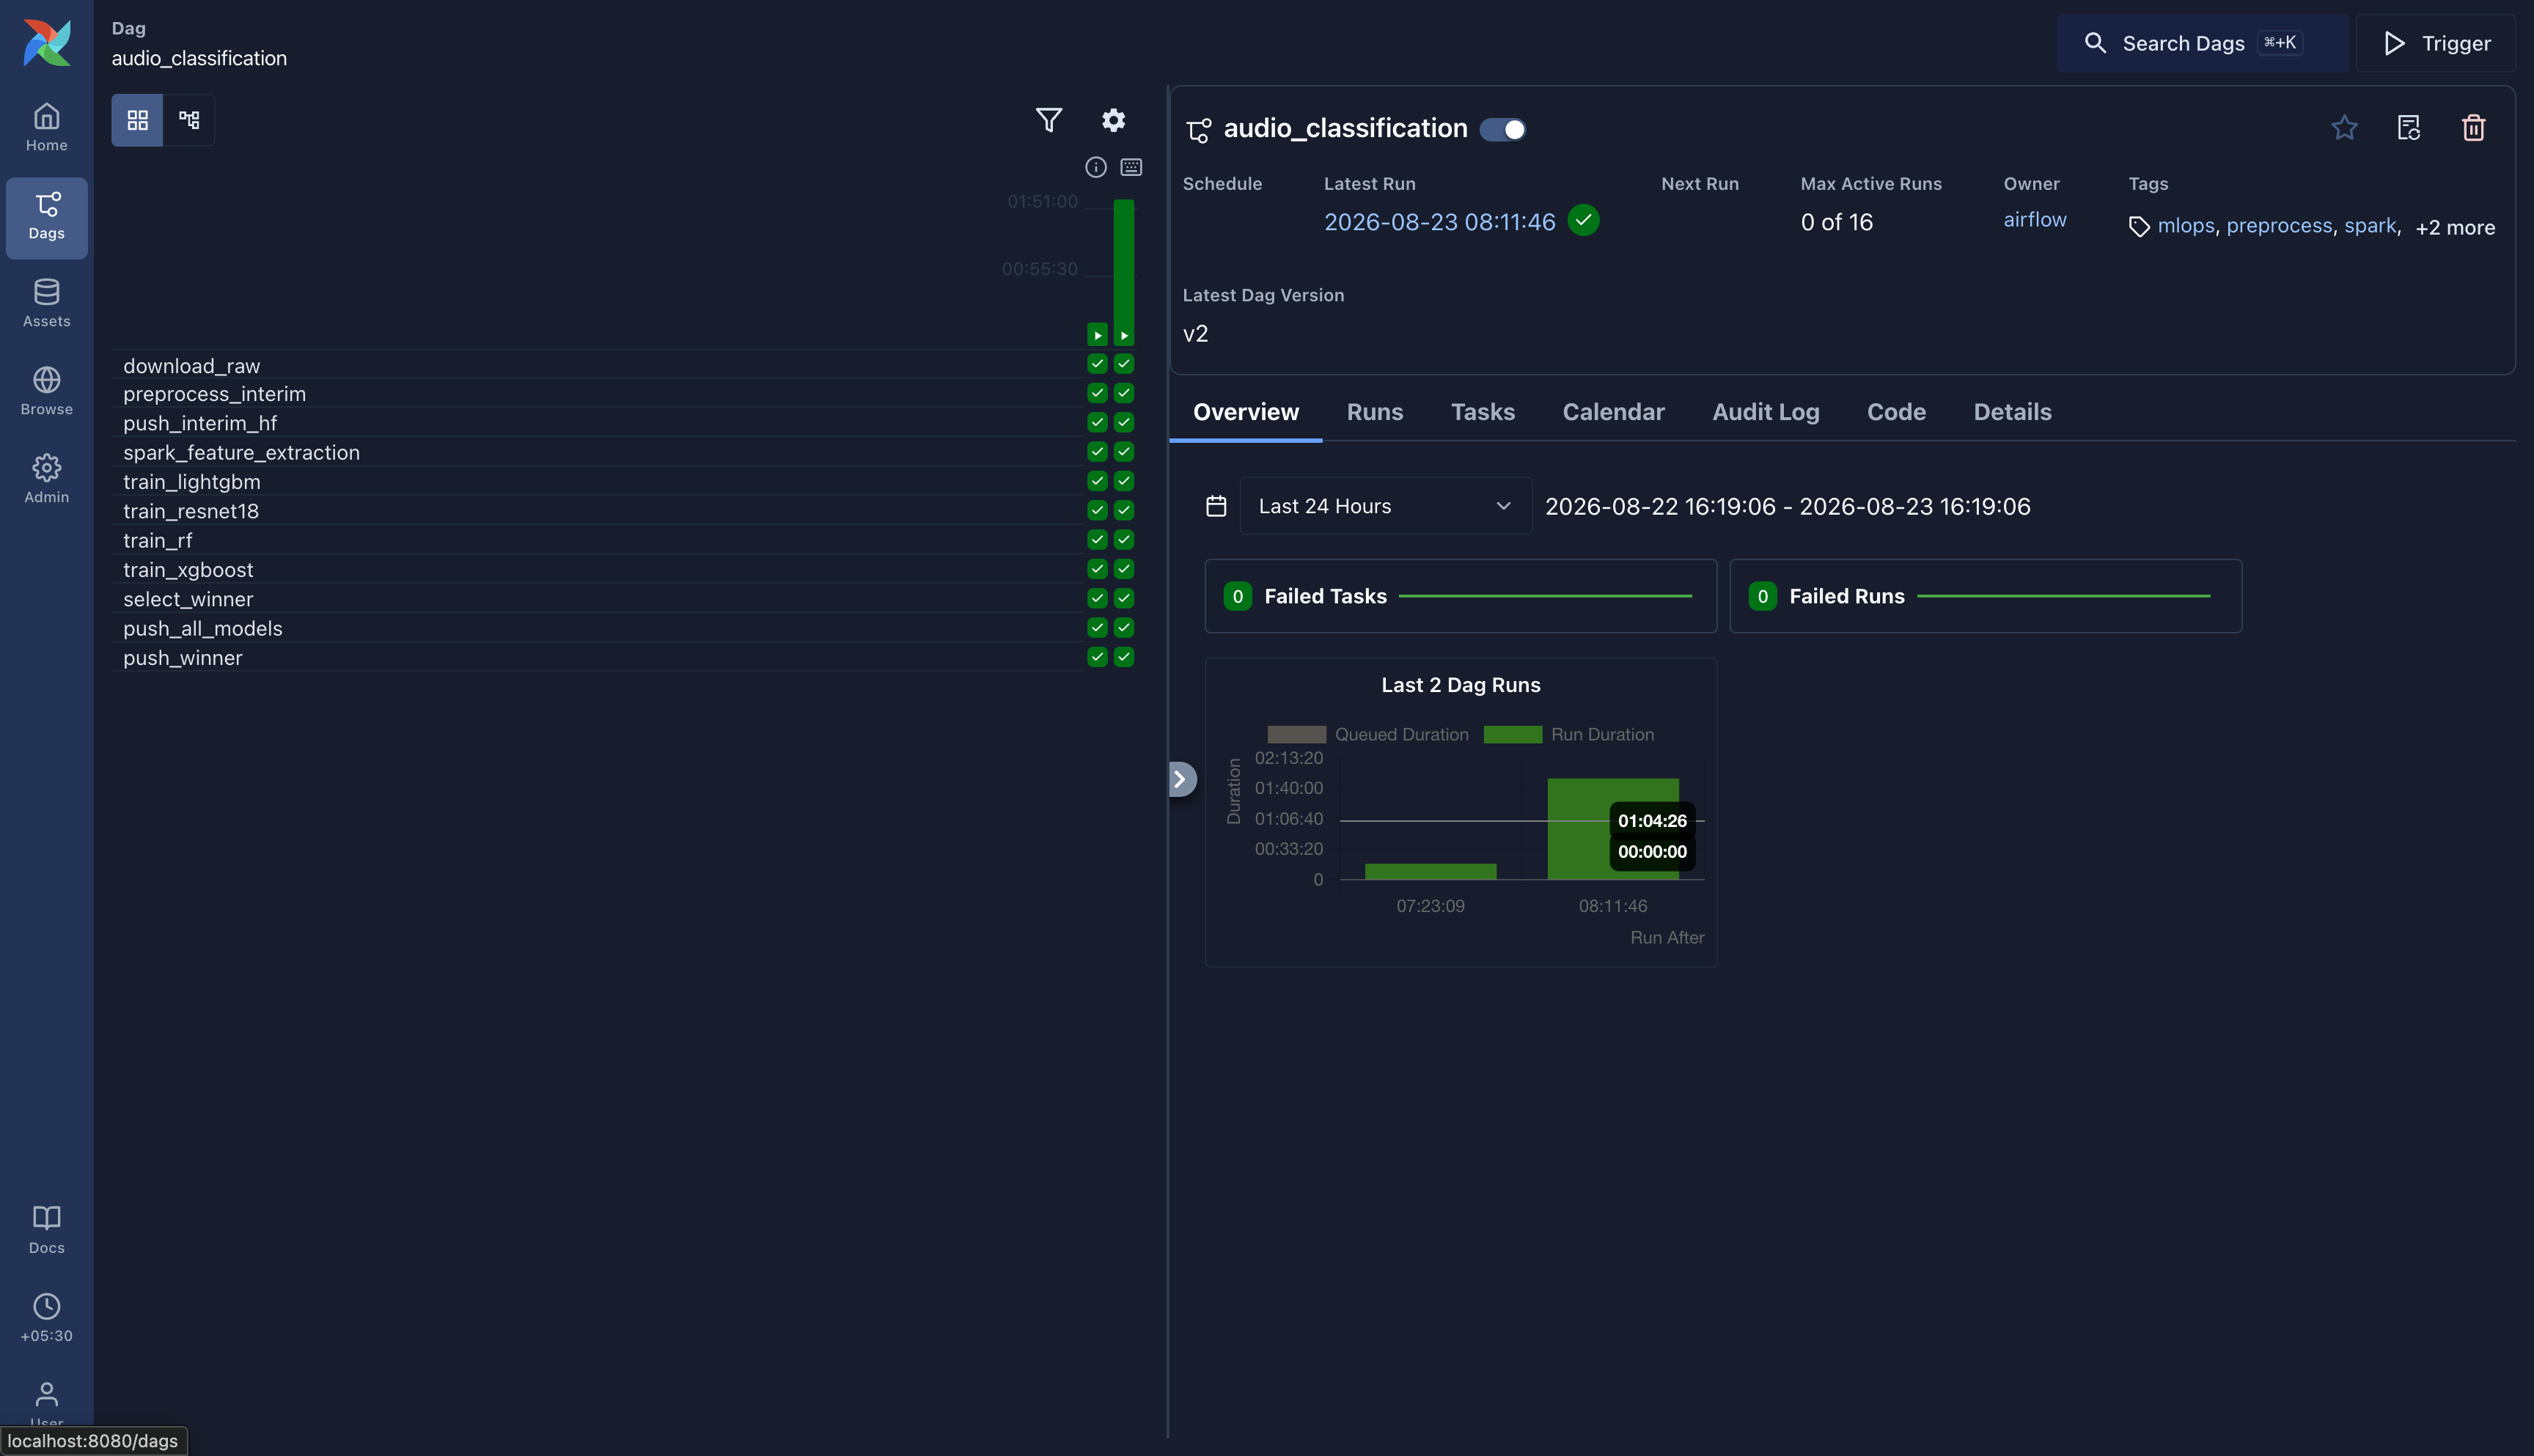
\includegraphics[width=\textwidth]{figures/airflow_runs_dashboard.png}
  \caption{Airflow DAG runs dashboard for \texttt{audio\_classification}. A manual trigger completed the full spine from dataset download through model pushes; parallel \texttt{train\_*} tasks reflect LocalExecutor fan-out on the host.}
  \label{fig:app-airflow}
\end{figure}

\clearpage
\begin{figure}[!t]
  \centering
  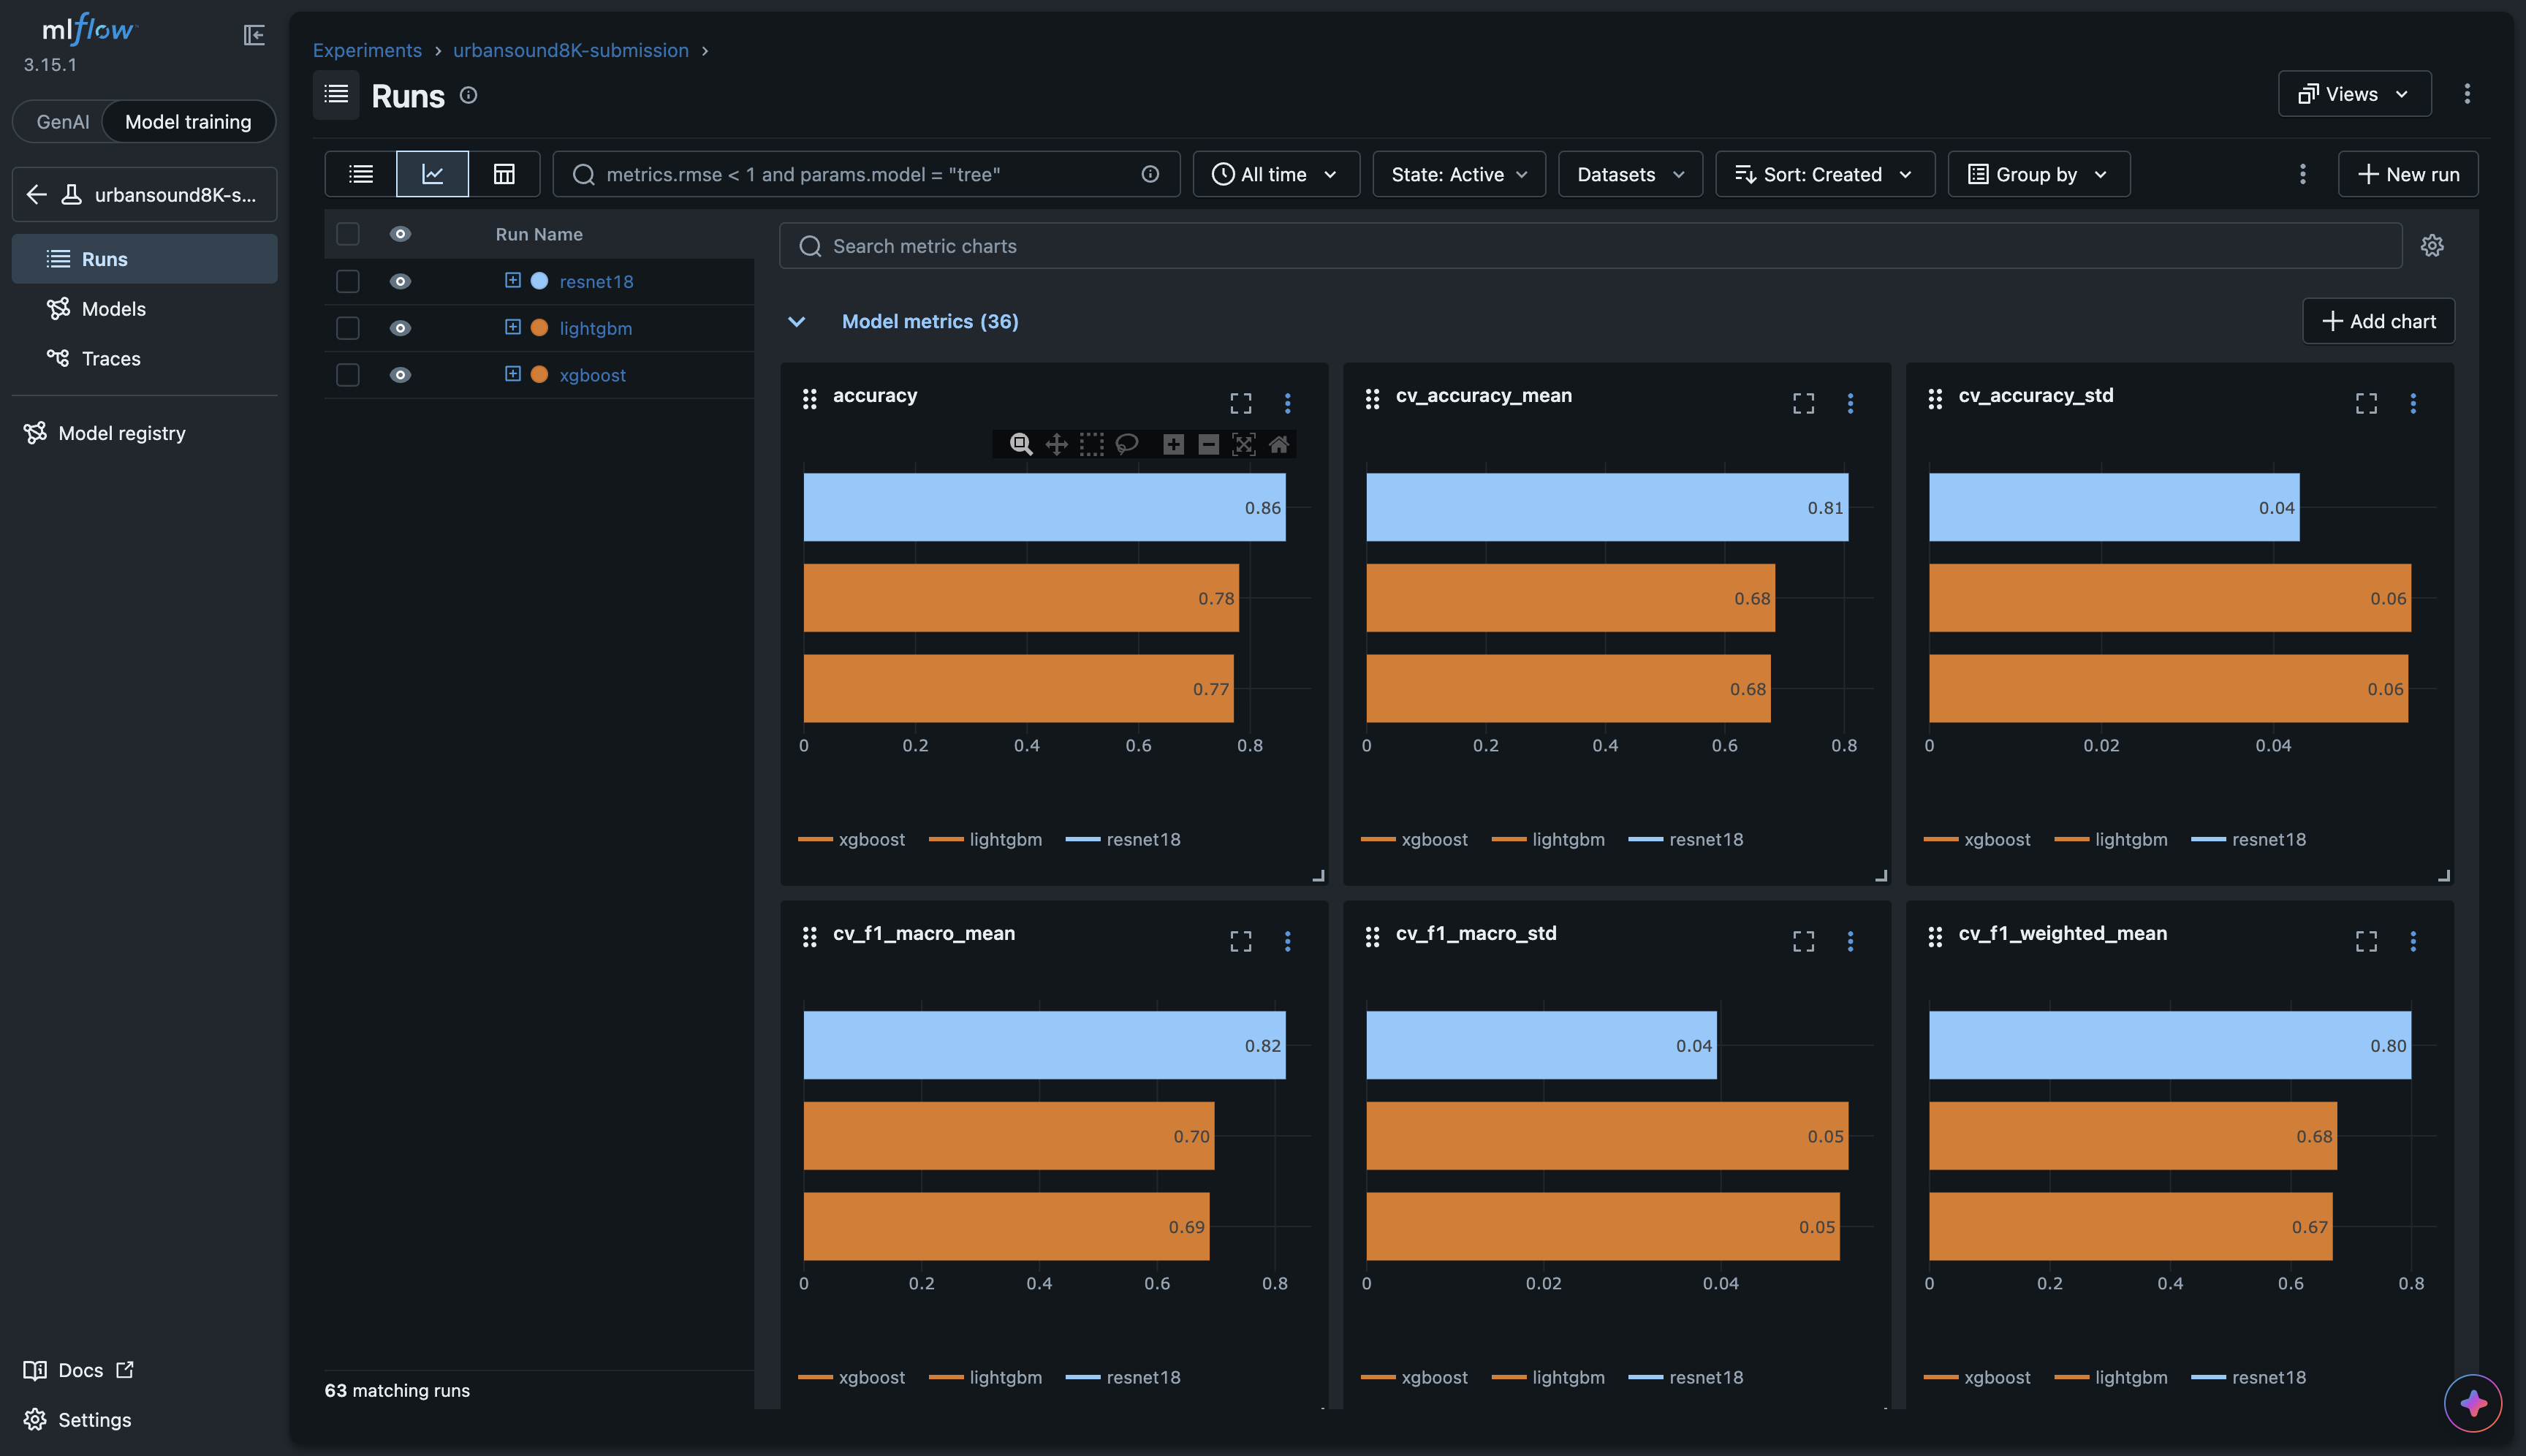
\includegraphics[width=\textwidth]{figures/mlflow.png}
  \caption{MLflow experiment runs for UrbanSound8K classification. Each run logs Optuna trials, fold-10 holdout metrics, optional 10-fold CV scores, confusion-matrix artifacts, and model binaries under a shared experiment name.}
  \label{fig:app-mlflow}
\end{figure}

\clearpage
\begin{figure}[!t]
  \centering
  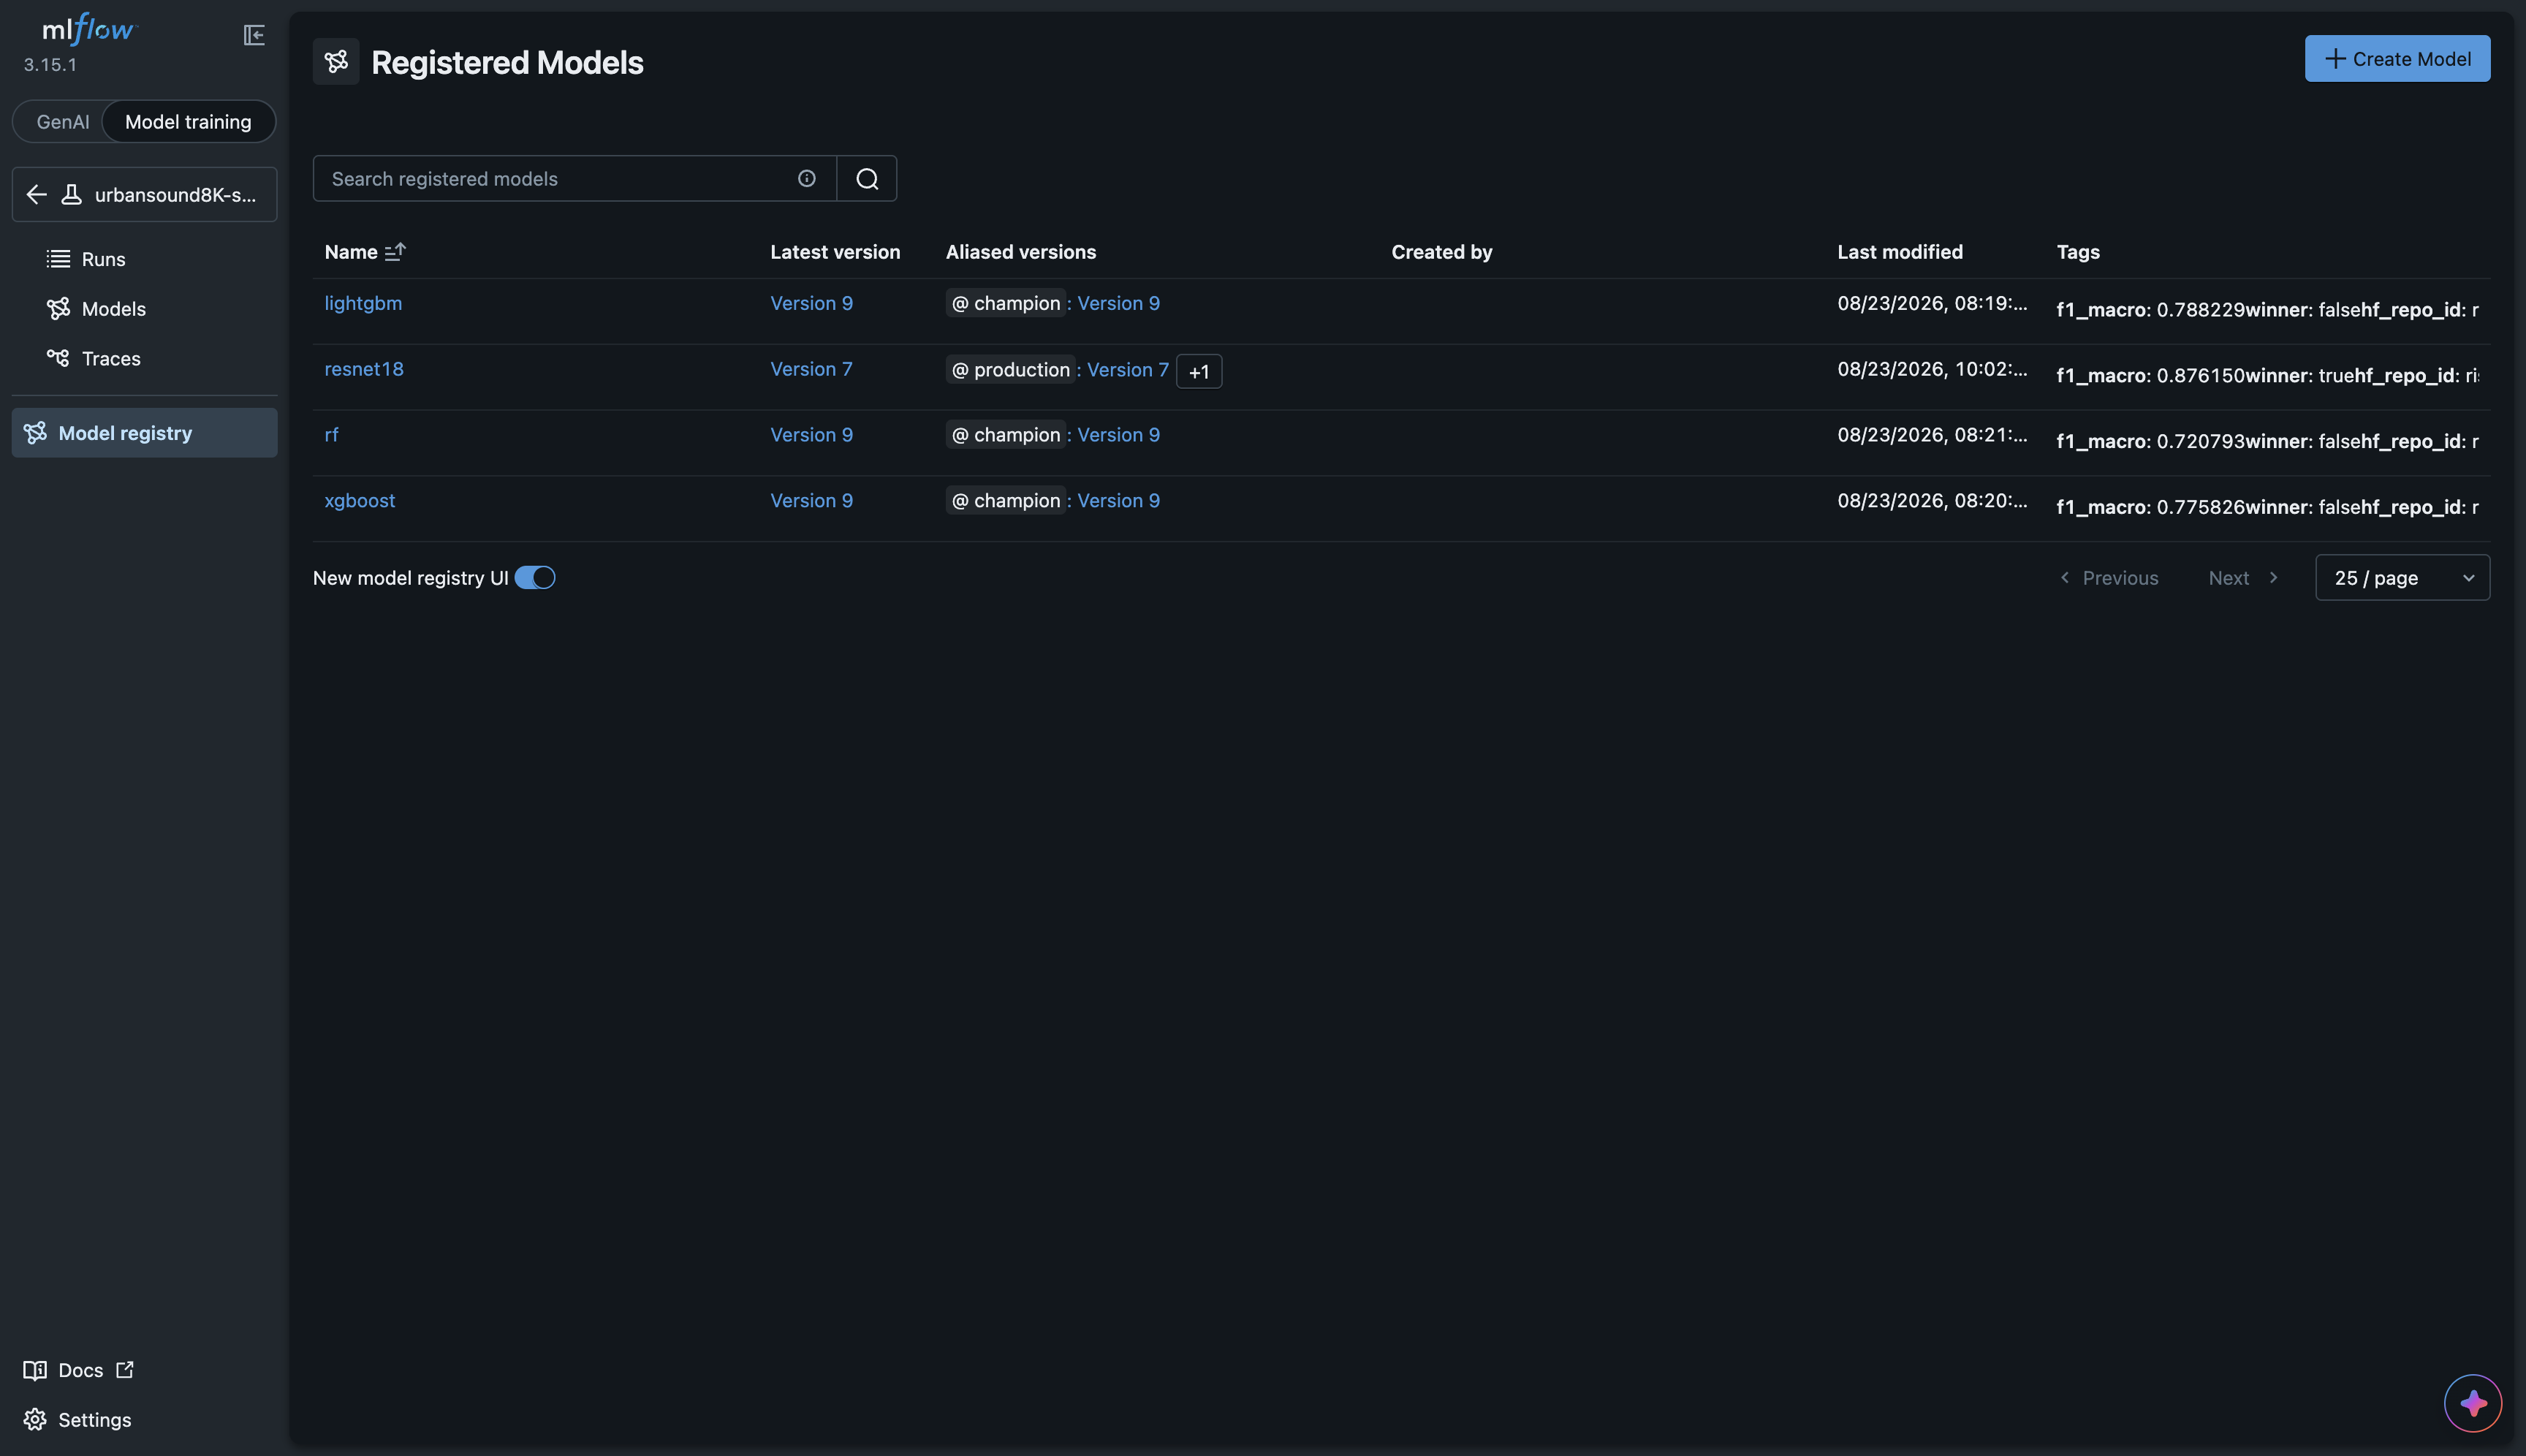
\includegraphics[width=0.92\textwidth]{figures/model_registry.png}
  \caption{MLflow Model Registry with the winning ResNet-18 promoted to the \texttt{Production} alias. Registry entries tie served weights to the MLflow \texttt{run\_id} recorded in \texttt{winner.json}.}
  \label{fig:app-registry}
\end{figure}

\clearpage
\begin{figure}[!t]
  \centering
  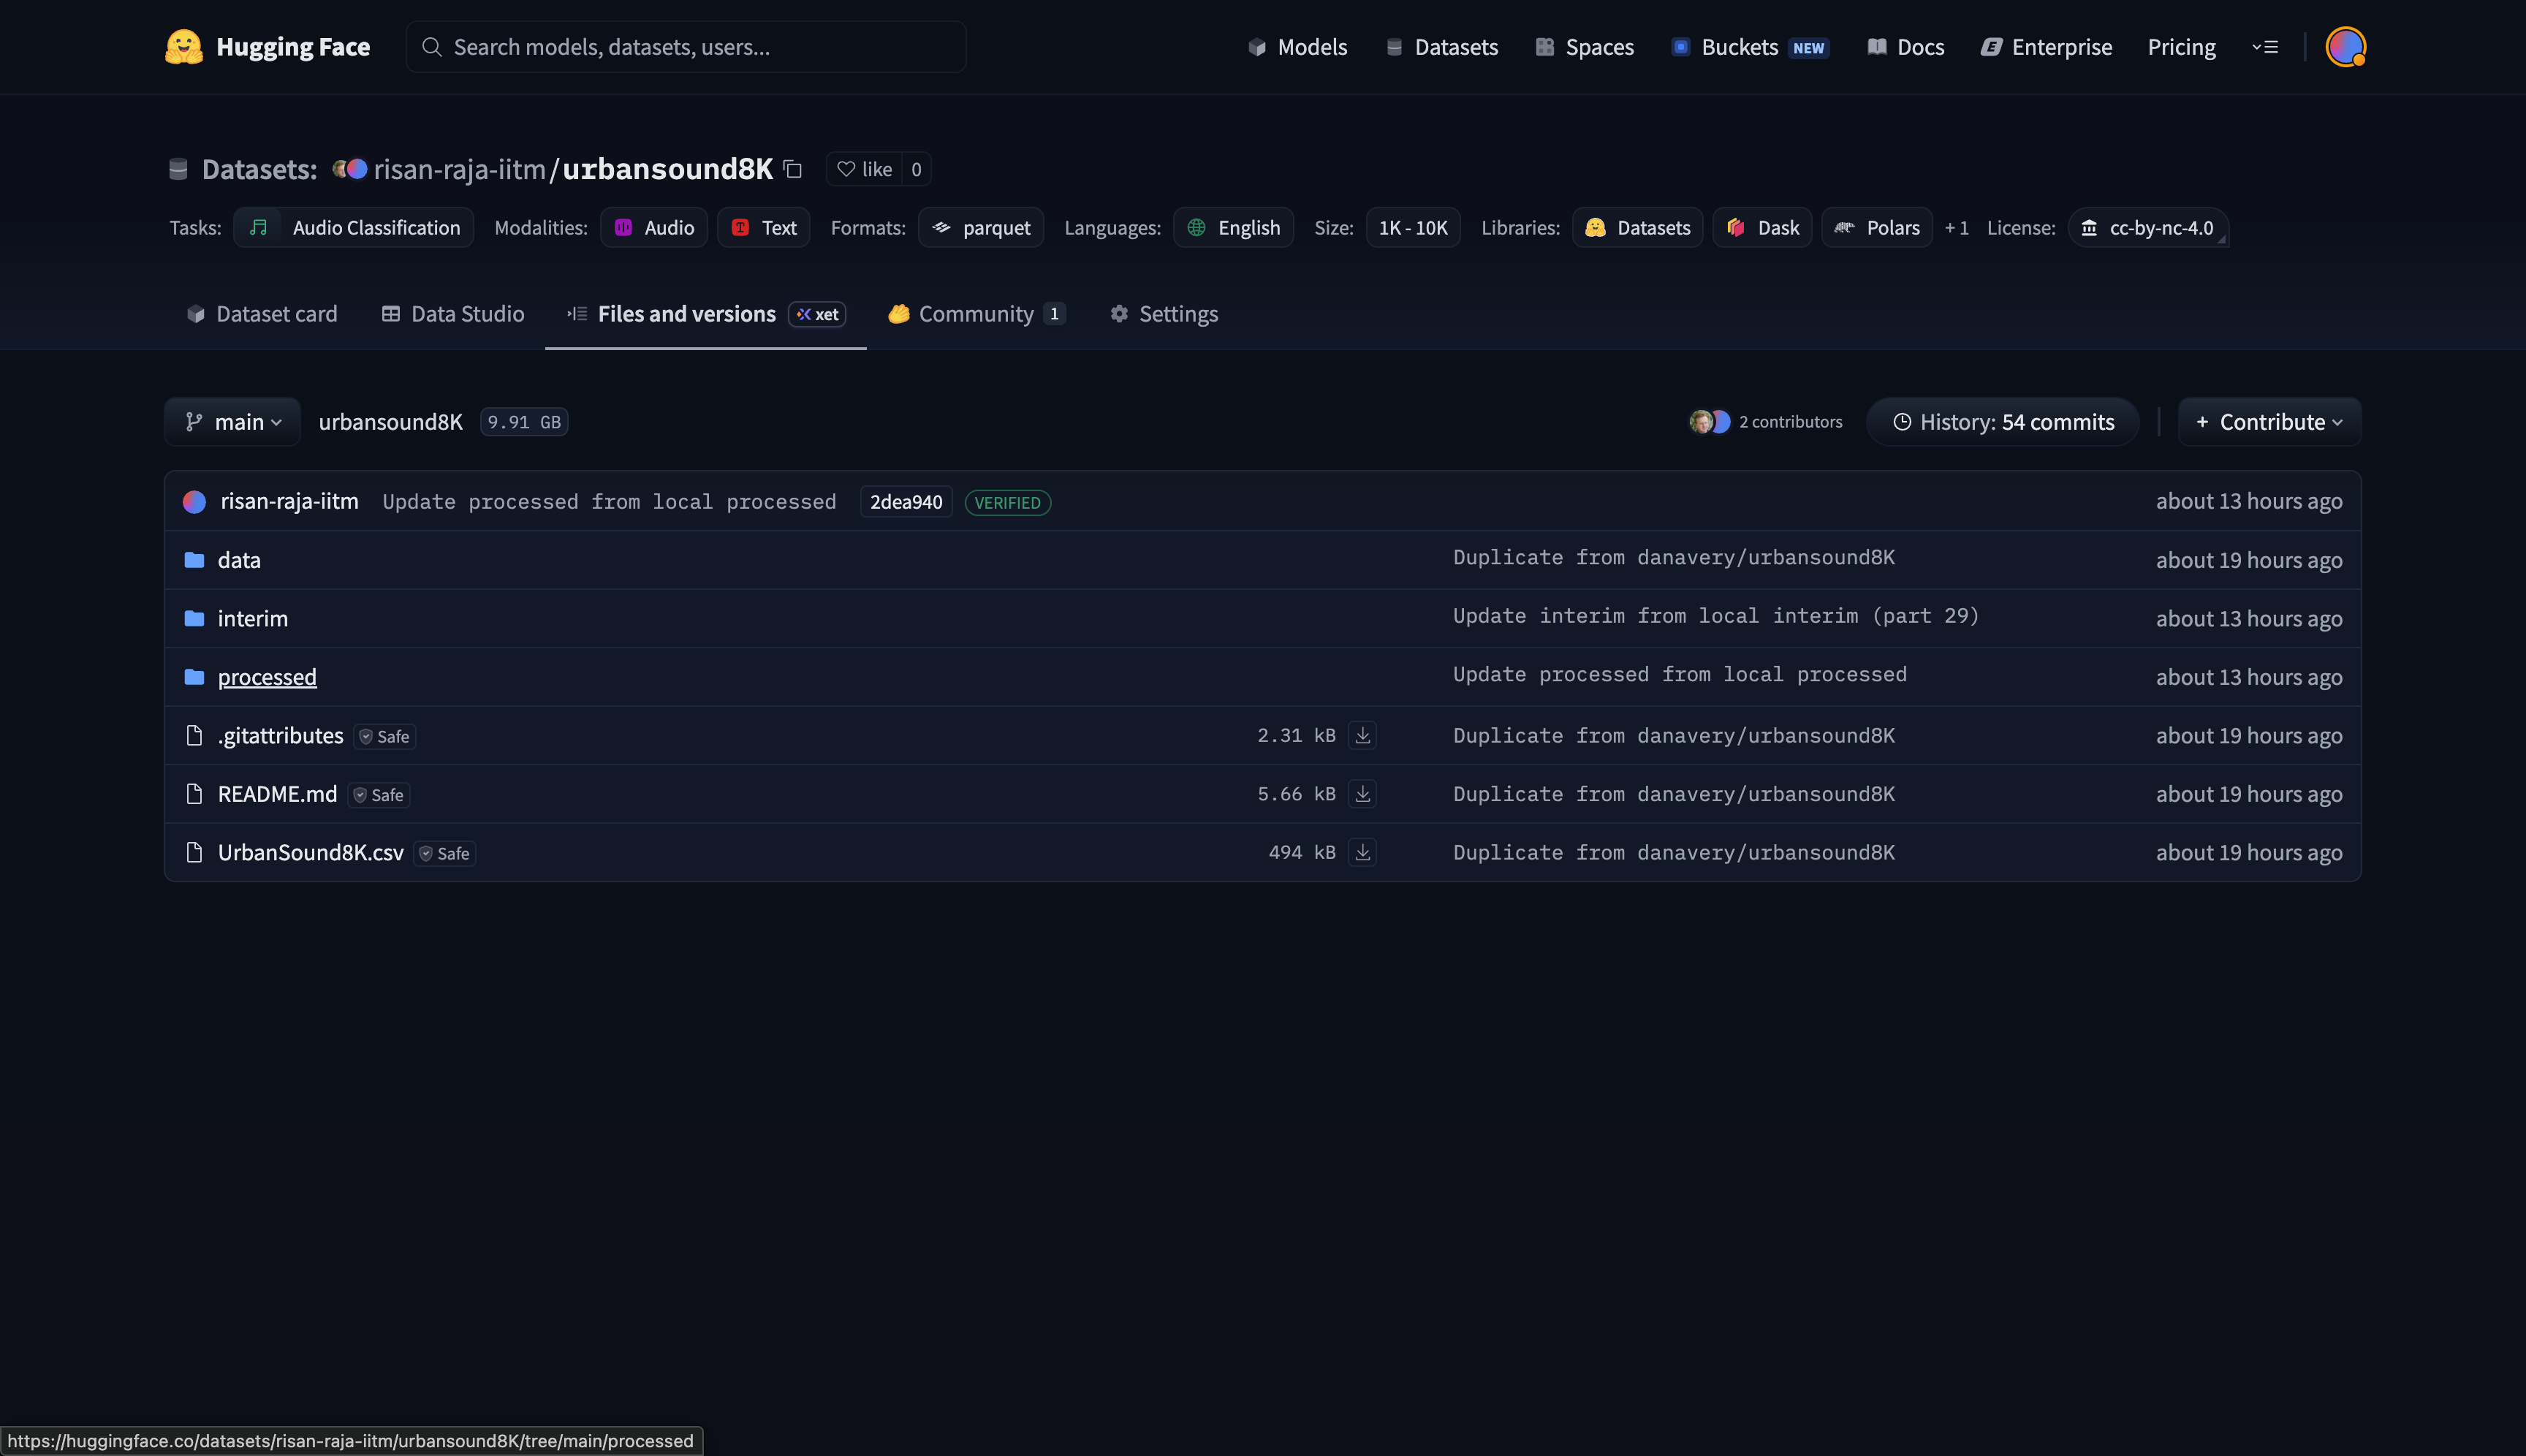
\includegraphics[width=\textwidth]{figures/hf_dataset_repo.png}
  \caption{Hugging Face dataset repository \dataset{risan-raja-iitm/urbansound8K}. Raw parquet remains upstream; pipeline outputs appear under \texttt{interim/} and \texttt{processed/} prefixes versioned by commit.}
  \label{fig:app-hf-dataset}
\end{figure}

\clearpage
\begin{figure}[!t]
  \centering
  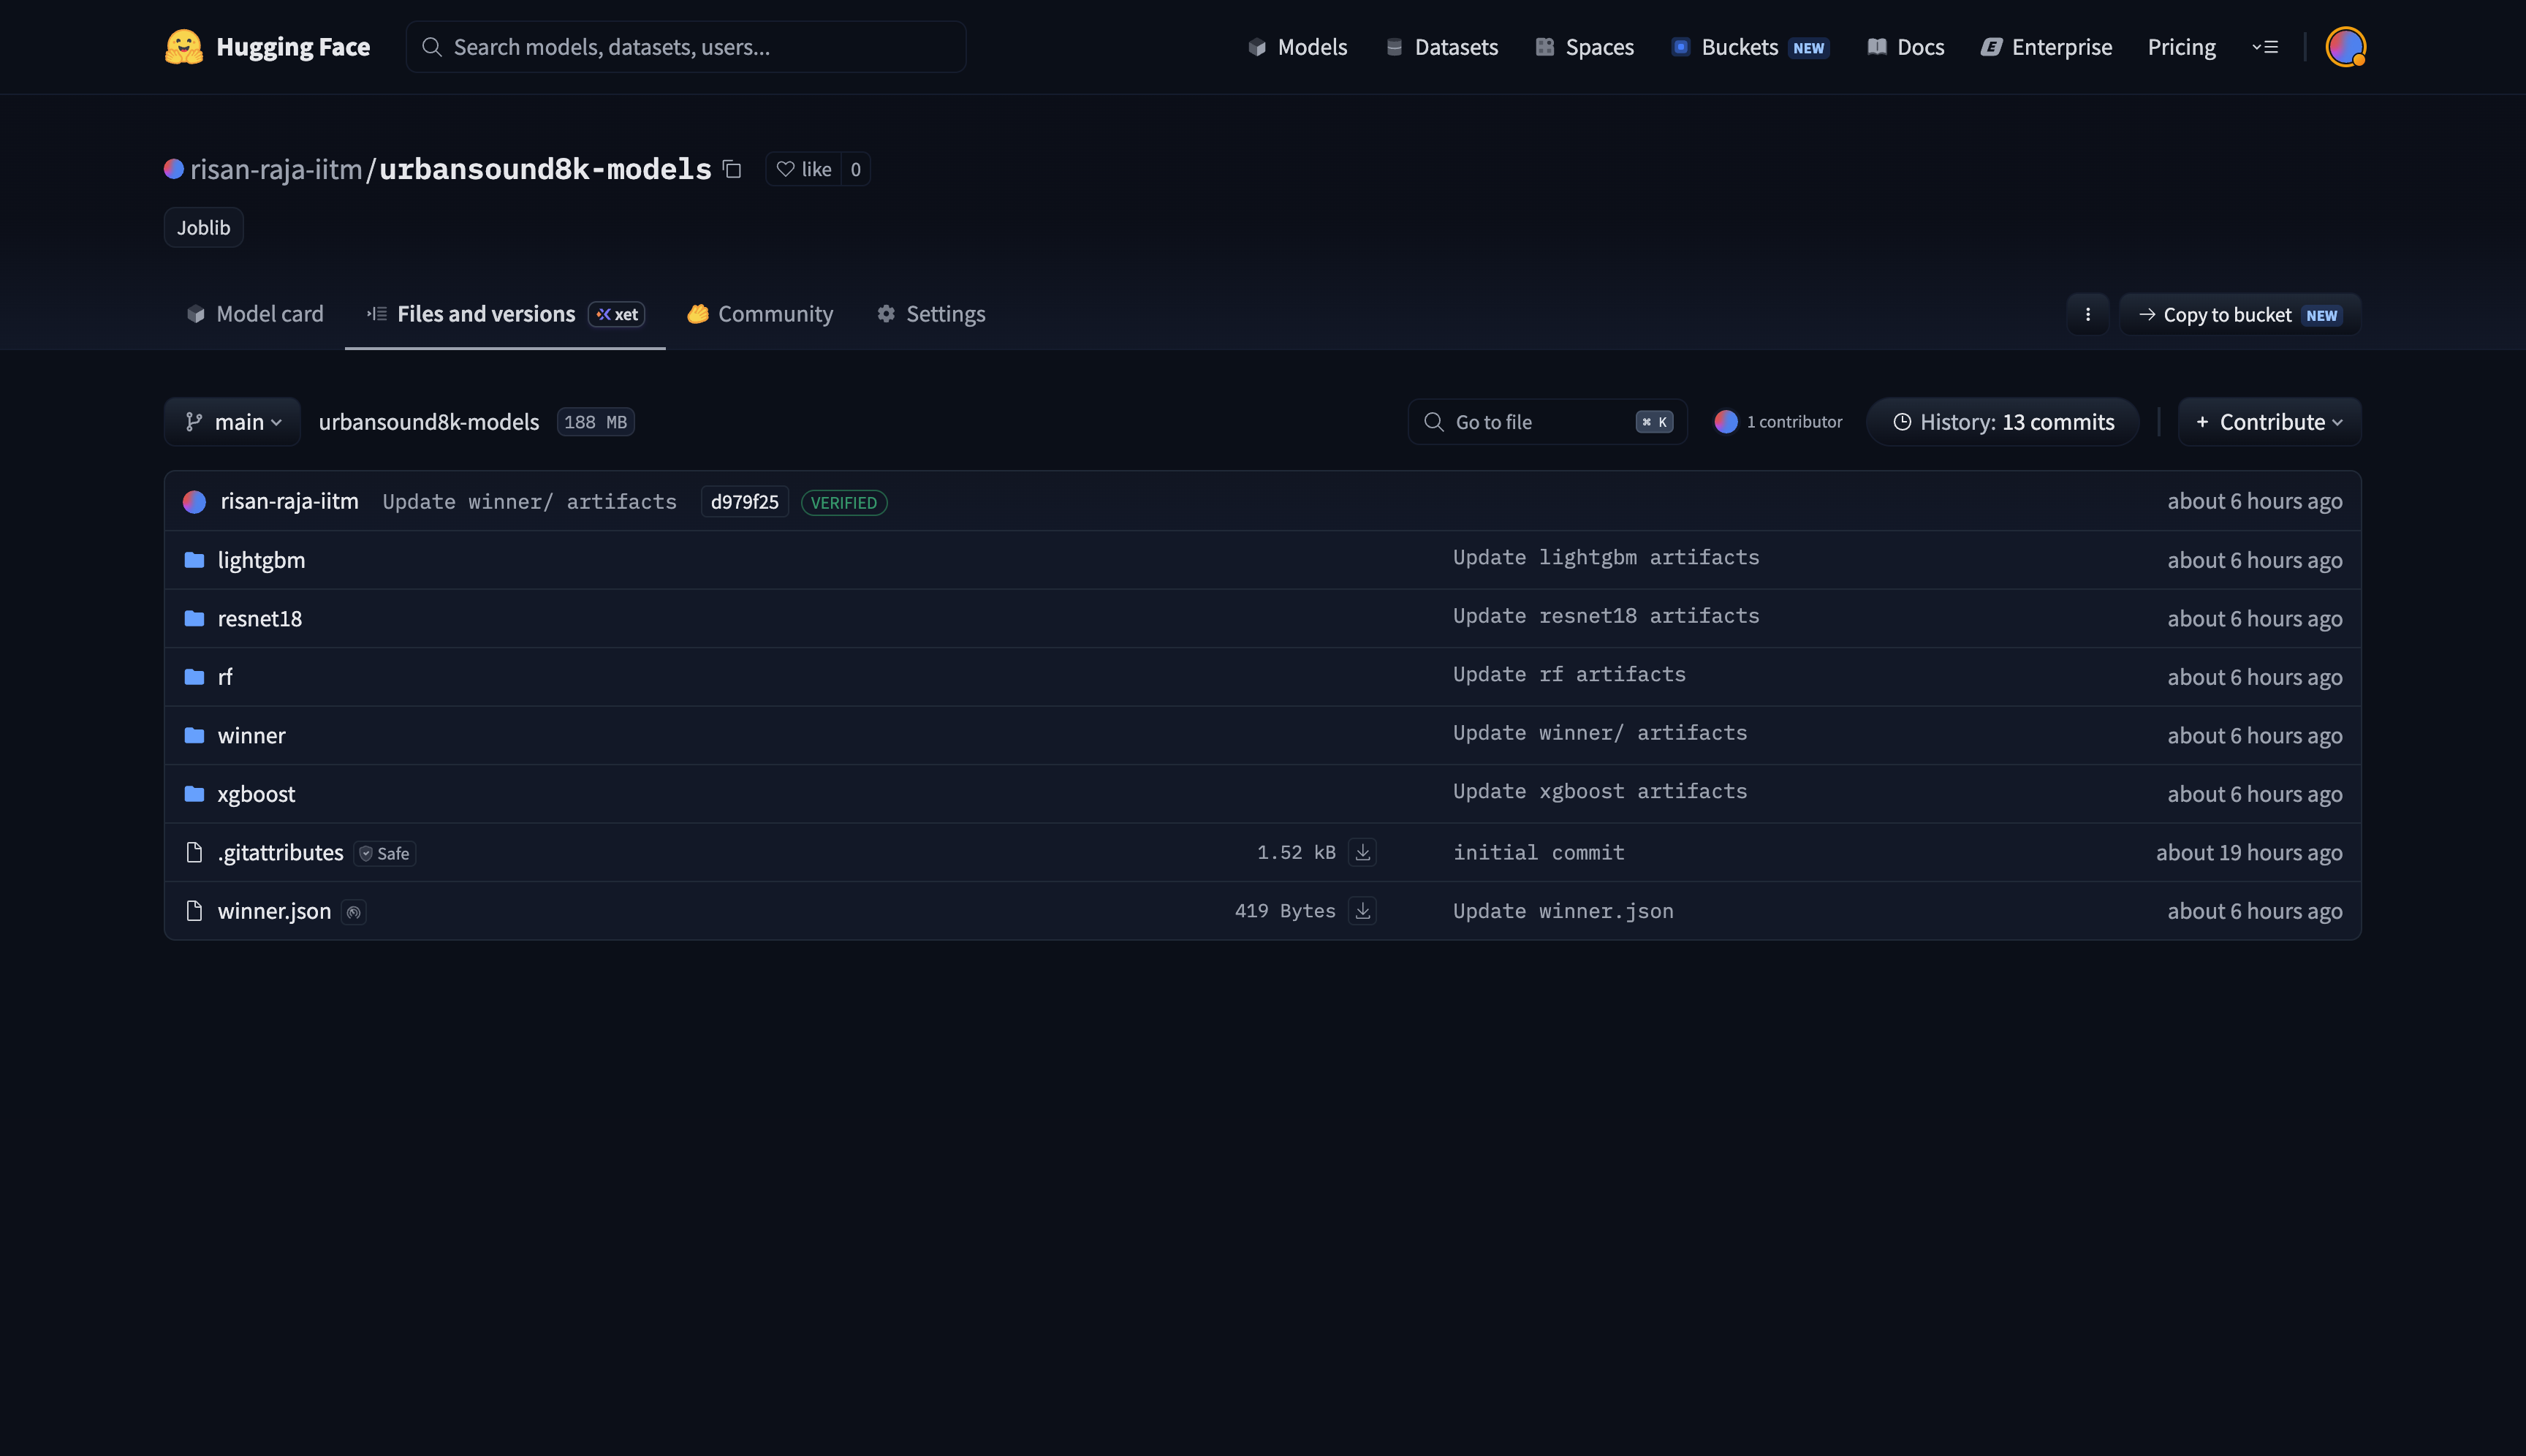
\includegraphics[width=\textwidth]{figures/hf_model_repo.png}
  \caption{Hugging Face model repository \dataset{risan-raja-iitm/urbansound8k-models}. Four trained directories, \texttt{winner.json}, and the \texttt{winner/} snapshot enable \texttt{make pull-winner} without a local retrain.}
  \label{fig:app-hf-model}
\end{figure}

\clearpage
\begin{figure}[!t]
  \centering
  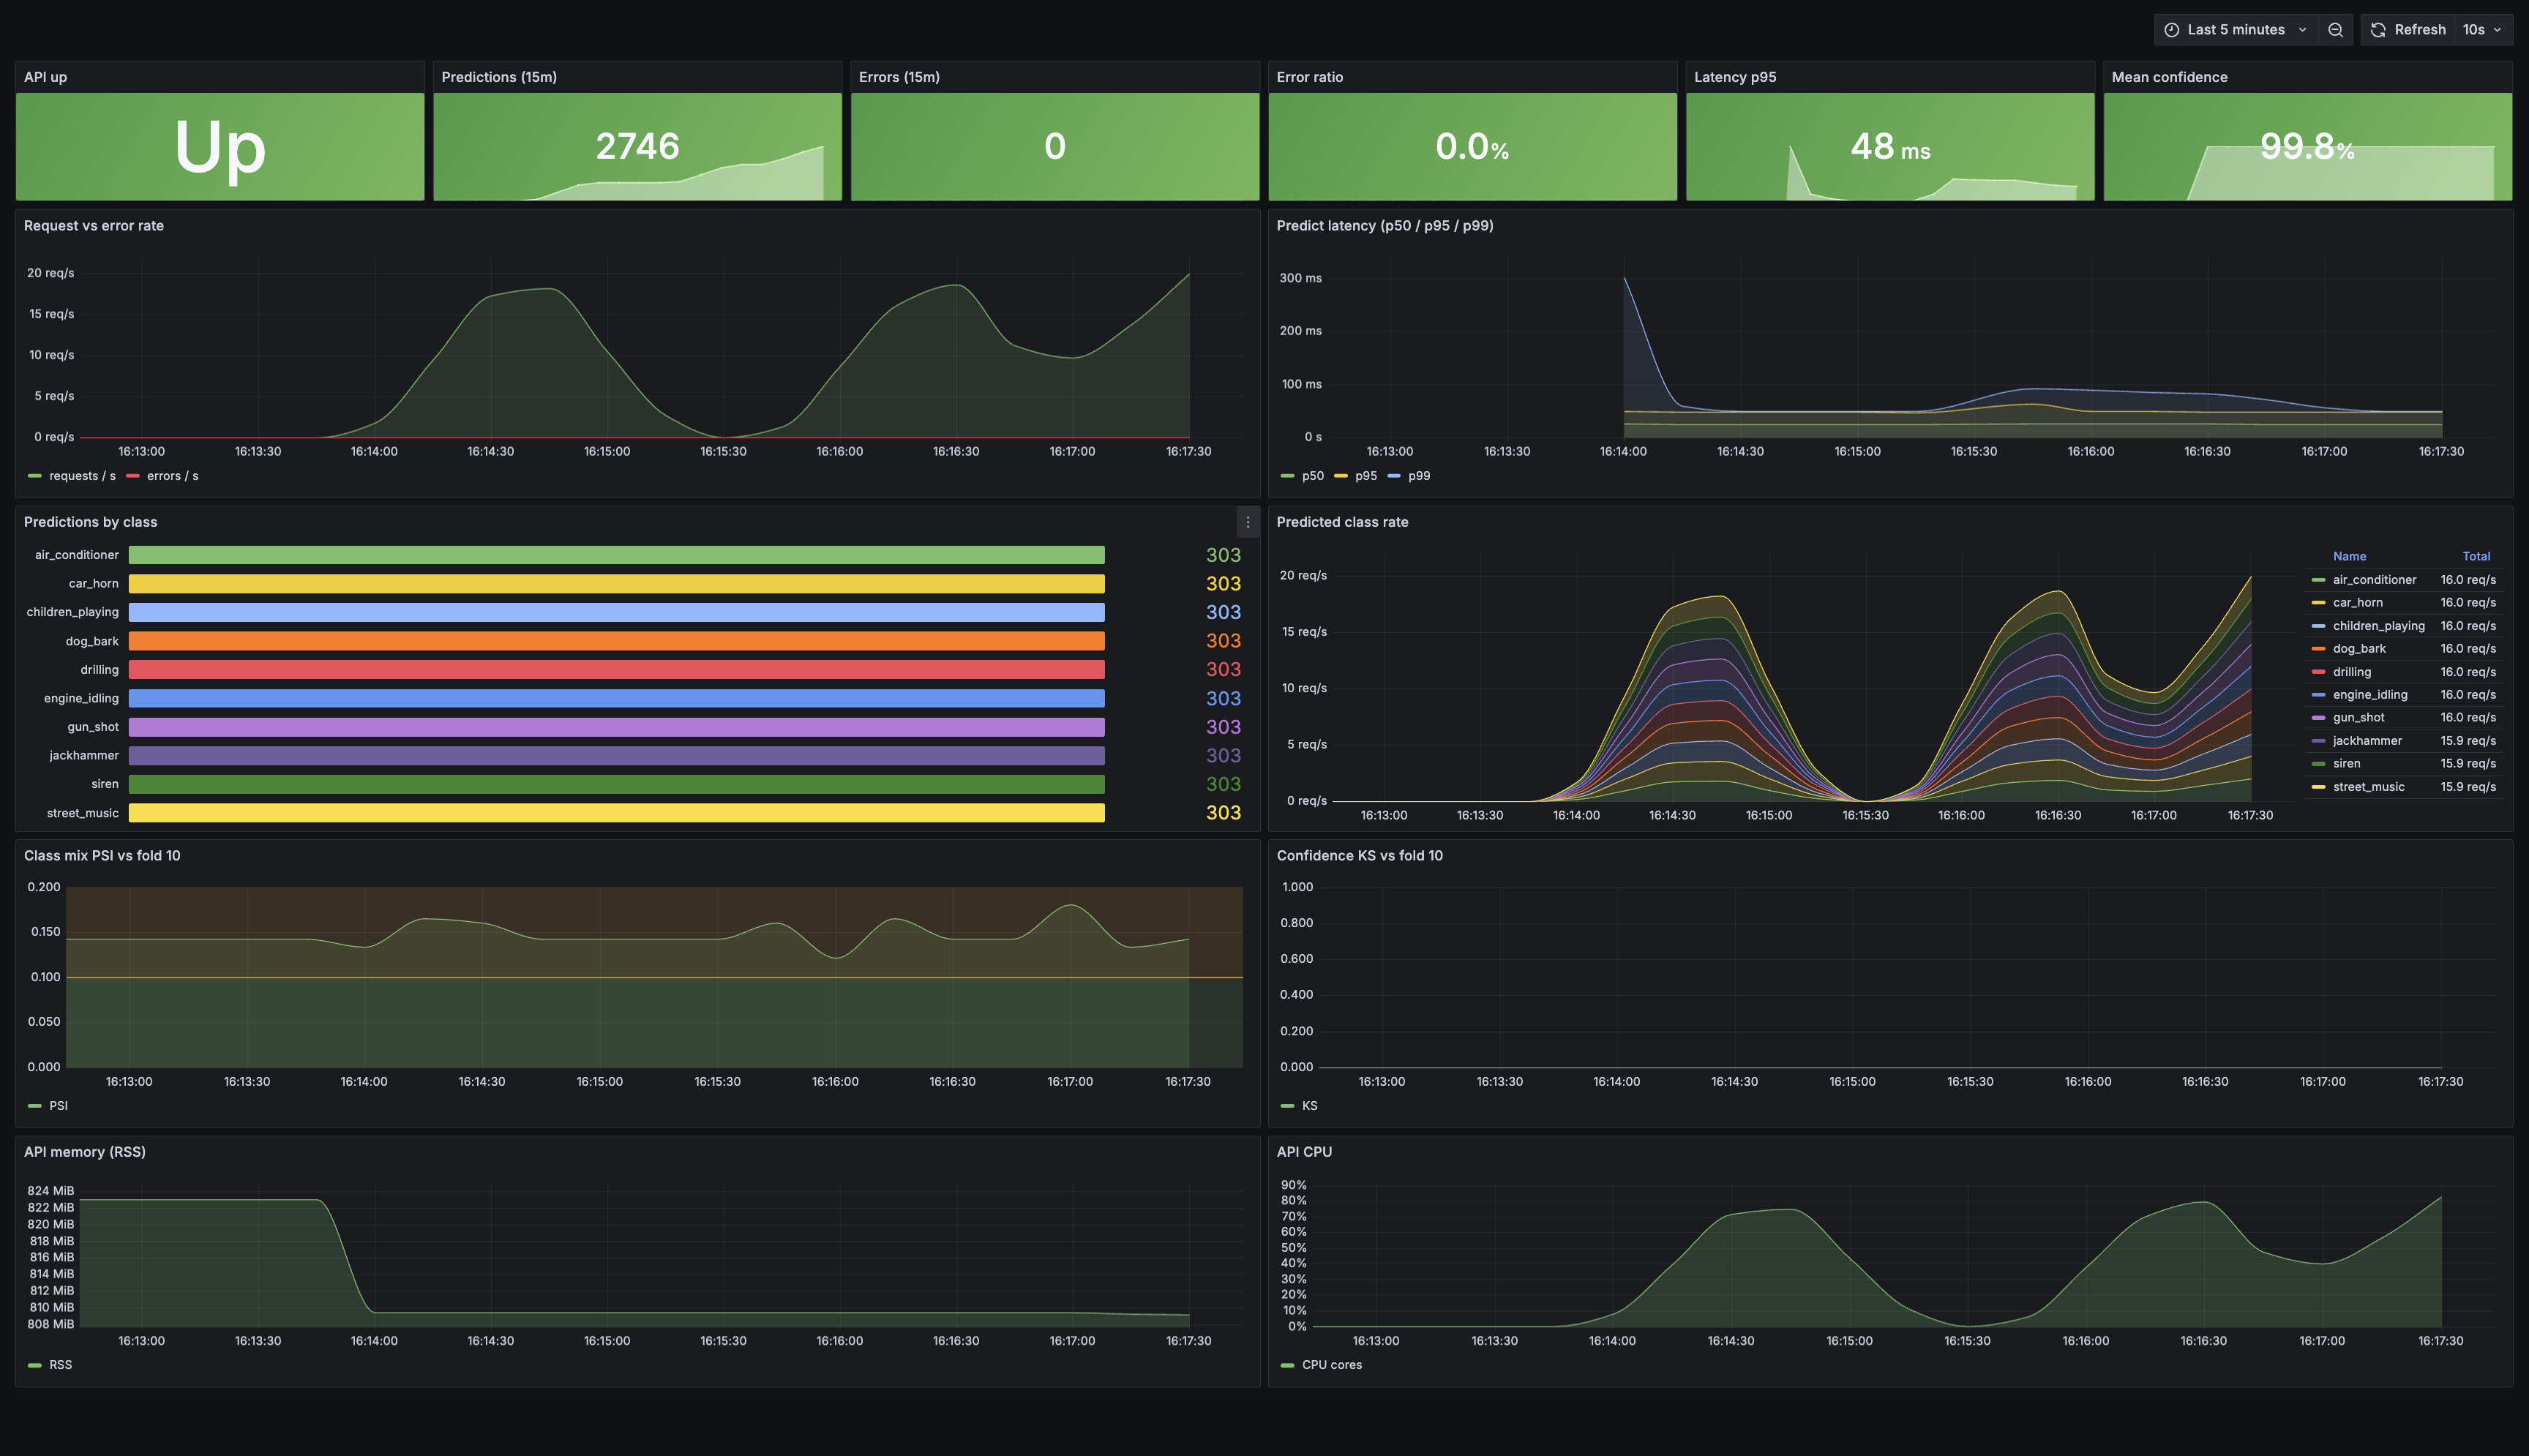
\includegraphics[width=\textwidth]{figures/grafana_dashboard.png}
  \caption{Grafana dashboard during demo traffic. Panels include request rate, error ratio, latency percentiles, predicted-class mix, mean confidence, and drift gauges (\texttt{drift\_psi\_class}, \texttt{drift\_ks\_confidence}) populated after \texttt{make demo-predict}.}
  \label{fig:app-grafana}
\end{figure}

\end{document}
